%% Black Cloud megacomputer toy model -- Acta Astronautica (Elsevier elsarticle) format.
%% One source, two typesettings, each built through a three-line wrapper that sets \papermode:
%%   submit.tex   -> submit.pdf    single column, 12 pt: the format Acta Astronautica requires for submission
%%   preprint.tex -> preprint.pdf  two columns (elsarticle 5p, Times): close to the published article
%% Build both:  latexmk -pdf submit preprint     (compiling main.tex directly gives the submission format)
\providecommand{\papermode}{submit}
\newif\iftwocol
\def\bcpreprintmode{preprint}\edef\bcgivenmode{\papermode}
\ifx\bcpreprintmode\bcgivenmode \twocoltrue \fi
\iftwocol
  \documentclass[final,5p]{elsarticle}
\else
  \documentclass[preprint,12pt]{elsarticle}
\fi

\usepackage[T1]{fontenc}
\usepackage{amsmath}
\iftwocol
  % 5p sets a 522 pt text width, leaving 37 pt side margins on A4; arXiv stamps its
  % identifier down the left margin, so narrow the text to clear it.
  \geometry{textwidth=486pt}
  \usepackage{newtxtext,newtxmath}   % Times text and math; newtxmath supplies the amssymb symbols
\else
  \usepackage{lmodern}
  \usepackage{amssymb}
\fi
\usepackage{microtype}
\usepackage{graphicx}
\usepackage{xcolor}
\usepackage{booktabs}
\usepackage{siunitx}
\usepackage[colorlinks=true,linkcolor=blue!50!black,citecolor=blue!50!black,urlcolor=blue!50!black]{hyperref}
\graphicspath{{../outputs/}}

\newcommand{\Lsun}{L_\odot}
\newcommand{\Mearth}{M_\oplus}
\newcommand{\kTl}{kT\ln 2}
\newcommand{\lcell}{\ell_{\rm cell}}
\newcommand{\todo}[1]{\textcolor{red}{[TODO: #1]}}

\journal{Acta Astronautica}

% Floats span the full page width in both layouts: one column in submit, both columns in preprint.
% Figures are drawn at the submit text width (5.4 in, plotstyle.py); in the wider preprint page they
% are printed at 407 pt (78% of the stock 5p text width) so their 9-10 pt labels stay at the size of
% the body text. Tables are scaled down only when they would not otherwise fit.
\newlength{\figwidth}
\newsavebox{\fitbox}
\iftwocol
  \setlength{\figwidth}{407pt}
  \newcommand{\fittable}[1]{\sbox{\fitbox}{#1}\ifdim\wd\fitbox>\textwidth\resizebox{\textwidth}{!}{\usebox{\fitbox}}\else\usebox{\fitbox}\fi}
\else
  \setlength{\figwidth}{\textwidth}
  \newcommand{\fittable}[1]{\resizebox{\textwidth}{!}{#1}}
\fi
% Single-panel figures with axes are drawn one stock 5p column wide (plotstyle.WC = 252 pt) and keep
% that width in the submit layout, so their 9-10 pt labels print at size. The narrowed preprint
% column is 234 pt, so there they fill the column at 93%.
\newlength{\colfigwidth}
\iftwocol
  \AtBeginDocument{\setlength{\colfigwidth}{\columnwidth}}   % the column width is set only by then
\else
  \setlength{\colfigwidth}{252pt}
\fi
\newenvironment{colfigure}{\begin{figure}[t]}{\end{figure}}
\iftwocol
  \newenvironment{widefigure}{\begin{figure*}[t]}{\end{figure*}}
  \newenvironment{widetable}{\begin{table*}[t]}{\end{table*}}
\else
  \newenvironment{widefigure}{\begin{figure}[t]}{\end{figure}}
  \newenvironment{widetable}{\begin{table}[t]}{\end{table}}
\fi

% Highlights are a submission item that the published article does not print: the preprint
% typesets them into a box that is thrown away.
\iftwocol
  \AtBeginDocument{\renewenvironment{highlights}{\setbox0=\vbox\bgroup\begin{itemize}}{\end{itemize}\egroup}}
\fi

% Short inline formulas never break at a relation or binary operator (see writing-style rule).
% The narrow columns of the preprint layout keep TeX's default penalties so lines can still fill.
\iftwocol
  \emergencystretch=3em
\else
  \relpenalty=10000
  \binoppenalty=10000
\fi

\begin{document}

\begin{frontmatter}

\title{Computing Cells, Signal Propagation and Technosignature Leakage in a Toy Model of a ``Black Cloud'' Megacomputer}

\author{James Guillochon}
\ead{guillochon@gmail.com}
\affiliation{Independent Researcher}

\begin{abstract}
Laughlin et al. (2021) proposed that a civilization could turn the dusty outflow of an asymptotic giant branch star into a ``Black Cloud'' computer: a shell about 220\,AU in radius at 150--200\,K, holding roughly an Earth mass of devices linked by millimeter-wave radio. We build a parametric toy model of such a machine to find how its signals propagate and what it leaks. The central result is the \emph{computing cell}, the largest region whose boundary bandwidth keeps pace with the bit operations inside it. For nodes that intercept starlight with covering $\tau$ and communicate over Fresnel-matched links of fractional bandwidth $f_B$, the cell size is $\ell_{\rm cell} = 2\tau f_B c\,kT\ln 2/(\beta F\lambda^2)$. Here $F$ is the absorbed flux, $\lambda$ the carrier wavelength and $\beta$ the bits exchanged per bit operation. The size is independent of lattice and shell thickness, so the carrier fixes the length, time and energy of a cell. Their 3\,mm links give 0.2\,mm cells between nodes 120\,km apart, and about $10^9$ times less bandwidth per operation than a supercomputer. For $\beta \sim 10^{-6}$ the optimum uses near-infrared links between centimeter-scale nodes 180\,m apart on a face-centered cubic lattice, which routes 20\% more efficiently than a 3D torus. The cloud is then about $10^{28}$ cells, each 1.8\,km across, ticking at about 50\,kHz and matching about half of El Capitan on 43\,W. Bolometric waste heat carries no information about the workload. Spectral width is a weaker discriminant against dust than usually assumed, but the sub-millimeter spectral index survives, and achromatic infrared variability marks a thermostatted design. Whole-star algorithms are limited to about $4\times10^5$ global supersteps. Internal communication is the only channel that carries computational state, and unresolved observers see cloud-wide activity smeared over $2R/c \approx 2.5$\,d.
\end{abstract}

\begin{highlights}
\item Computing-cell size scales as $1/(\beta F\lambda^2)$, set by the carrier wavelength.
\item Millimeter links leave a Black Cloud about $10^{9}$ times short of needed bandwidth.
\item Optimal clouds use near-IR links, 180\,m node spacing and FCC (high-radix) lattices.
\item Waste heat traces the star; only the comm band carries computational state.
\item Light travel smears frame-synchronous activity into a $2R/c\approx2.5$\,d boxcar.
\end{highlights}

\begin{keyword}
technosignatures \sep SETI \sep Dyson spheres \sep AGB stars \sep Landauer limit \sep interconnection networks
\end{keyword}

\end{frontmatter}

%======================================================================
\section{Introduction}
%======================================================================

Searches for waste heat from technological civilizations go back to \citet{Dyson1960}. In the WISE era they have been formalized by the \^G survey \citep{Wright2014a,Wright2014b,Wright2019} and by Project Hephaistos \citep{Suazo2022,Suazo2024}. These searches rest on energy conservation: any civilization that uses a large fraction of its star's luminosity must re-radiate it, usually in the mid-infrared. Their weak point is confusion with dusty astrophysical sources. The seven Hephaistos M-dwarf candidates have been attributed to background dust-obscured galaxies \citep{Ren2024,Blain2024}, and JWST has confirmed this directly for two of them \citep{Zackrisson2026}.

\citet{LaughlinAdams2021} considered a sharper version of the waste-heat argument. They noted that if Earth's computing keeps growing at its present rate, its power demand will exceed the sunlight that the planet intercepts within about a century. They then asked where device-based computation could be carried out on a larger scale, and argued that the cool, metal-rich winds of AGB stars are a natural site. The star supplies the energy, and the outflow supplies carbonaceous and silicate condensates that could be assembled into nanoscale devices communicating wirelessly at millimeter wavelengths. For a shell that re-radiates the stellar luminosity, the Landauer-limited rate \citep{Landauer1961,Bennett1982,Lloyd2000} grows as $R^{1/2}$. \citet{LaughlinAdams2021} therefore placed the shell at the largest radius at which water ice does not coat the grains, where the temperature falls to about 150\,K. For a host of $1000\,\Lsun$ this gives a structure about 220\,AU in radius that performs $3\times10^{50}$ bit operations per second. It holds about $1\,\Mearth$ of carbon and silicates and is rebuilt roughly every 300\,yr as the wind carries it away. They call such objects ``Black Clouds,'' after the novel by \citet{Hoyle1957}. Black Clouds would appear as luminous, nearly blackbody sources at 150--200\,K. \citet{LaughlinAdams2021} searched the WISE catalog for sources with colors close to those of a prototype in the Large Magellanic Cloud and found 208, concentrated in the Galactic disk toward the Galactic center. They also proposed that ejected devices might survive in presolar grains in meteorites, and that their carbon-rich ejecta might show up in the diffuse interstellar bands as molecular populations far from chemical equilibrium. \citet{ScharfWitkowski2024} generalize the argument to ``computational zones,'' which likewise predict cool far-infrared emitters.

\citet{LaughlinAdams2021} also estimated how fast a Black Cloud can communicate. They argued that dust absorbs wavelengths shorter than about 1\,mm and that wavelengths longer than about 1\,cm carry too little bandwidth, and adopted a 3\,mm carrier. Channels of 1\,cm$^2$ covering a shell 500\,AU in radius, each carrying $10^{10}$\,bit\,s$^{-1}$, give a total of $7\times10^{42}$\,bit\,s$^{-1}$. That is about $10^8$ times less than the computing rate. Since a signal takes hours to cross the structure, they concluded that a Black Cloud must operate in a massively parallel fashion. Two aspects of this proposal have not, to our knowledge, been modeled quantitatively. The first is how information moves \emph{inside} such a structure, and how large a region can compute as one. The second is whether anything that leaks out carries information about the computation itself rather than about the star's energy budget. Time-domain signatures in particular are almost absent from the waste-heat literature, which works with static spectral energy distributions (SEDs). They are, however, the basis of a complementary strand of SETI that looks for information written into stellar variability. \citet{Learned2008} proposed encoding a galactic beacon in the pulsation phases of Cepheids, and \citet{Guillochon2026} searched 77{,}596 pulsating stars for such codes. That search found no beacon. It also noted that a perfectly compressed message is indistinguishable from noise, so a civilization communicating efficiently rather than advertising could escape every timing test. Here we ask the complementary question for a machine that is \emph{not} trying to be seen: what does efficient internal communication unavoidably leak?

Terrestrial supercomputers offer a useful template. Their interconnects are meshes and tori embedded in physical space: three-dimensional tori in Blue Gene/L \citep{Adiga2005}, a six-dimensional mesh/torus in the K computer and Fugaku \citep{Ajima2009,Ajima2018}, a two-dimensional on-wafer mesh in wafer-scale engines \citep{Lie2024}, and hierarchical dragonfly \citep{Kim2008} or fat-tree \citep{Leiserson1985} networks that add long links between groups. Their design is governed by the ratio of communication to computation and by Rent's rule. According to that rule, the number of terminals of a block of $g$ gates scales as $g^{p}$ with $p<1$ \citep{Landman1971,Christie2000}, so a block's communication grows more slowly than its computation. We carry this reasoning over to an astrophysical computer and find that it defines a natural \emph{computing cell} whose size, timescale, energy and frequency are tied to the carrier wavelength.\footnote{An interactive, not-to-scale rendering of the fiducial design is available at \url{https://blackcloud.astrocrash.net}. It runs from the whole shell and its backbone down to one cell, one node and the minds that it hosts.}

Section~\ref{sec:model} describes the toy model. Section~\ref{sec:cells} derives the computing cell and the optimal three-dimensional structure. Section~\ref{sec:workloads} describes the algorithms suited to each level of the resulting hierarchy. Section~\ref{sec:results} presents propagation, thermal and leakage results, and Section~\ref{sec:discussion} discusses observing strategy and limitations.

\begin{widetable}
\centering
\caption{Fiducial parameters. Every quantity is a free parameter of the accompanying code. The stellar and wind values lie within the ranges reviewed by \citet{HofnerOlofsson2018}, and the pulsation amplitude is derived in \S\ref{sec:host}. The remaining entries are design choices.}
\label{tab:params}
\small
\fittable{\begin{tabular}{lll}
\toprule
Symbol & Meaning & Fiducial value \\
\midrule
$L_\ast$, $T_\ast$ & mean stellar luminosity, effective temperature & $2000\,\Lsun$, 2800\,K \\
$P_{\rm Mira}$, $\delta L$ & pulsation period, fractional semi-amplitude & 400\,d, 0.4 \\
$R$, $M_{\rm c}$ & outer radius, mass of the structure & 220\,AU, $1\,\Mearth$ \\
$f_{\rm c}$, $\tau$ & covering fraction, radial covering optical depth & 0.995, 1 \\
$v_{\rm exp}$ & outflow speed & $10\,\si{km.s^{-1}}$ \\
$\nu_{\rm c}$, $B$ & millimeter communication band (Laughlin--Adams case) & 100\,GHz, 10\,GHz \\
$f_B$ & fractional link bandwidth & 0.1 \\
$a$, $a_{\rm hub}$ & mesh-node and backbone-hub aperture sides (\S\ref{sec:results}) & 20\,m, 10\,km \\
$\tau_{\rm p}$ & relay latency per hop & 1\,ms (sub-mm), 1\,$\mu$s (cells) \\
$\eta_{\rm max}$ & maximum power fraction spent on local links & 0.01 \\
$m$ & link margin above the Shannon limit & 2 \\
\bottomrule
\end{tabular}}
\end{widetable}

%======================================================================
\section{Model}\label{sec:model}
%======================================================================

\subsection{Host and structure}\label{sec:host}
The host is a Mira-type AGB star \citep{HofnerOlofsson2018} with luminosity
\iftwocol\predisplaypenalty=0 \fi   % preprint: let the column break before this display, so the section can start at the foot of a column
\begin{equation}
L_\ast(t)=\bar L_\ast\left[1+\delta L\sin(2\pi t/P_{\rm Mira})\right].
\end{equation}
\iftwocol\predisplaypenalty=10000 \fi
Miras are defined by visual amplitudes of 2.5 to 11\,mag \citep{Samus2017}. The 1.25\,$\mu$m band lies close to the flux peak of a 2800\,K photosphere (1.03\,$\mu$m by Wien's law), so its amplitude is a proxy for the bolometric amplitude. At that wavelength, Mira light curves vary by 0.20\,mag per magnitude of visual variation \citep{Smith2002}. A visual amplitude of 2.5 to 5\,mag therefore implies 0.5 to 1.0\,mag, or a luminosity semi-amplitude $(10^{0.4\Delta m}-1)/(10^{0.4\Delta m}+1)$ of 0.23 to 0.43. We adopt $\delta L=0.4$. We treat the computer as a spherically symmetric shell of outer radius $R$ that intercepts a fraction $f_{\rm c}$ of the starlight. In radiative equilibrium its outer surface has the temperature
\begin{equation}
T = \left(\frac{f_{\rm c}L_\ast}{4\pi\sigma R^2}\right)^{1/4} = 177\,{\rm K}\left(\frac{L_\ast}{2000\,\Lsun}\right)^{1/4}\left(\frac{R}{220\,{\rm AU}}\right)^{-1/2}.
\end{equation}
\citet{LaughlinAdams2021} adopted $1000\,\Lsun$, for which a shell of 220\,AU sits at the 150\,K ice limit. We keep their radius but take a host twice as luminous, which raises the shell to 177\,K. The absorbed flux per unit area of shell is $F=f_{\rm c}L_\ast/4\pi R^2=55\,\si{W.m^{-2}}$. Spreading $M_{\rm c}=1\,\Mearth$ over the shell gives an areal mass of $\Sigma=0.44\,\si{g.m^{-2}}$.

\subsection{Thermodynamic budget}
If all absorbed power is dissipated at $T$, the rate of irreversible bit operations is $\dot N_{\rm L} = f_{\rm c}L_\ast/\kTl = 4.5\times10^{50}\,{\rm bit\,s^{-1}}$. Blackbody radiation carries entropy $4/3$ of its energy divided by its temperature, so the entropy budget of the radiation, with light arriving at $T_\ast$ and leaving at $T$, gives the slightly larger bound $\tfrac43 f_{\rm c}L_\ast(T^{-1}-T_\ast^{-1})/(k\ln2)=5.6\times10^{50}\,{\rm bit\,s^{-1}}$. \citet{LaughlinAdams2021} instead treated each computing layer as a Carnot engine between a hot inner reservoir at $T_{\rm h}$ and its own outer surface at $T$. Their rate carries an extra factor $(T_{\rm h}-T)/(T_{\rm h}+T)$, about 1/2 for the ratio $T_{\rm h}/T\approx3$ that they expected from the opacities of the grains. We use $\dot N_{\rm L}$, the limit of their result for $T_{\rm h}\gg T$, so our throughputs are upper bounds by up to that factor. The radiative time constant of the film is
\begin{equation}
\tau_{\rm th} = \frac{\Sigma\,c_p}{8\sigma T^3}\le 0.36\,{\rm s}.
\end{equation}
The bound uses the Dulong--Petit heat capacity of carbon, $3R$ per mole or $2.1\,\si{kJ.kg^{-1}.K^{-1}}$, which the true heat capacity at 177\,K cannot exceed. Even the bound is negligible compared with every other timescale in the problem.

\subsection{Links}
A link between apertures $A_t$ and $A_r$ a distance $d$ apart obeys the Friis relation \citep{Friis1946}, capped at unity inside the near field:
\begin{equation}
\mathcal{L}(d) = \max\!\left[1,\ (\lambda d)^2/A_tA_r\right].
\end{equation}
For $d\le A/\lambda$ two apertures share about one orthogonal spatial mode, or more at shorter range \citep{Miller2000}. A phase-insensitive (coherent) receiver with thermal occupation $\bar n=(e^{h\nu/kT}-1)^{-1}$ has a noise floor of $h\nu(\bar n+1)$ per mode \citep{Caves1982}, so we charge
\begin{equation}
E_{\rm bit}(\nu) = m\,\ln2\,\frac{h\nu}{1-e^{-h\nu/kT}} + \kTl.
\label{eq:ebit}
\end{equation}
The first term reduces to the low-SNR Shannon limit $m\,\kTl$ in the Rayleigh--Jeans regime \citep{Shannon1948} and to $m\,h\nu\ln2$ in the quantum regime. The second term adds about $\kTl$ for each decoding and re-encoding at a relay.

\subsection{Observer}
Let $\hat n$ be the direction to the observer and $\mathbf{x}_i$ the unit position vector of a shell element. Emission at cloud time $t$ arrives at observed time $t_{\rm obs} = t - (R/c)\,\mathbf{x}_i\cdot\hat n$. By Archimedes' hat-box theorem, $\mathbf{x}\cdot\hat n$ is uniformly distributed on $[-1,1]$ over a uniform sphere. A modulation that is simultaneous in the cloud frame is therefore convolved with a boxcar of width $2R/c$, and its Fourier amplitude is multiplied by
\begin{equation}
H(f) = \left|\operatorname{sinc}\!\left(2fR/c\right)\right| = \left|\frac{\sin(2\pi fR/c)}{2\pi fR/c}\right|.
\label{eq:transfer}
\end{equation}

%======================================================================
\section{Computing cells and the optimal three-dimensional structure}\label{sec:cells}
%======================================================================

\subsection{Node density from starlight covering}
We place nodes on a three-dimensional lattice that fills a shell of thickness $\Delta R$. Each node is a convex body of surface $S$ whose mean projected area is $S/4$ (Cauchy's theorem). Requiring radial covering $\tau$ of the starlight therefore fixes the surface density of nodes:
\begin{equation}
nS = \frac{4\tau}{\Delta R},
\end{equation}
where $n$ is the number density. Following terrestrial mesh networks, every node carries one port per nearest neighbor. Here a port is a flat aperture of area $A$, so $S=zA$ for coordination number $z$. The natural node shape is the lattice's Wigner--Seitz cell, whose faces point at the neighbors (Fig.~\ref{fig:lattices}). Matching each link at the Fresnel distance ($d=A/\lambda$: one mode, no path loss) and writing the nearest-neighbor distance as $d=\kappa n^{-1/3}$ gives
\begin{equation}
d = \kappa^{3/2}\sqrt{\frac{z\lambda\Delta R}{4\tau}},\qquad A=\lambda d,\qquad N_z=\frac{\Delta R}{d}.
\label{eq:spacing}
\end{equation}

\begin{colfigure}
\centering
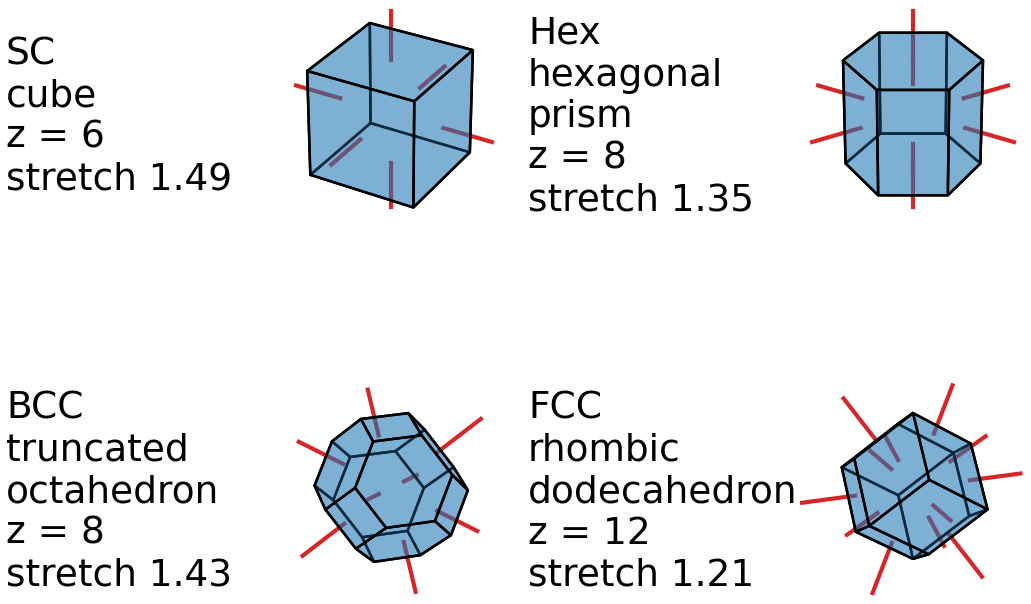
\includegraphics[width=\colfigwidth]{fig8_lattices.png}
\caption{Candidate node lattices (simple cubic, simple hexagonal, body-centered and face-centered cubic) and their Wigner--Seitz node shapes, with one aperture per nearest neighbor (red); $z$ is the coordination number. The routing stretch is the mean ratio of shortest-path length on the lattice graph to Euclidean distance.}
\label{fig:lattices}
\end{colfigure}

\begin{widetable}
\centering
\caption{Lattice comparison. $\kappa=d\,n^{1/3}$; $\hat\sigma$ is the number of links crossing a plane per unit area in units of $n^{2/3}$ (orientation average and worst case); the stretch is computed by breadth-first search on a $19^3$ block.}
\label{tab:lattices}
\small
\fittable{\begin{tabular}{llcccccl}
\toprule
Lattice & Node shape & $z$ & $\kappa$ & stretch & $\hat\sigma$ (mean/min) & Terrestrial analog \\
\midrule
SC  & cube & 6 & 1.000 & 1.49 & 1.50 / 1.03 & 3D torus \citep{Adiga2005} \\
Hex & hexagonal prism & 8 & 1.049 & 1.35 & 2.10 / 1.10 & stacked 2D meshes \citep{Lie2024} \\
BCC & truncated octahedron & 8 & 1.091 & 1.43 & 2.18 / 1.79 & 8-port diagonal mesh \\
FCC & rhombic dodecahedron & 12 & 1.122 & 1.21 & 3.37 / 2.80 & high-radix mesh \citep{Ajima2009} \\
\bottomrule
\end{tabular}}
\end{widetable}

\subsection{The bandwidth-balanced cell}
Each Fresnel-matched link carries $b=f_B\nu$ bits per second. The bisection bandwidth per unit area of a plane cutting the lattice is $\hat\sigma n^{2/3}b$. Substituting Eq.~\eqref{eq:spacing}, $z$ and $\kappa$ cancel to within the orientation factor:
\begin{equation}
\sigma_b \simeq \frac{\tau f_B c}{\Delta R\,\lambda^2}.
\end{equation}
The bit-operation density is $\dot c_v = F/(\Delta R\,\kTl)$. Consider a region of linear size $\ell$ that computes $\dot c_v\ell^3$ bit operations per second and, in the spirit of Rent's rule \citep{Landman1971,Christie2000}, needs to exchange a fraction $\beta$ of them with the rest of the machine. Its boundary can supply that traffic only up to the size at which $\ell^2\sigma_b=\beta\dot c_v\ell^3/2$:
\begin{equation}
\boxed{\;\lcell = \frac{2\tau f_B\,c\,\kTl}{\beta\,F\,\lambda^2}\;}
\label{eq:lcell}
\end{equation}
The same expression holds for a column $\ell\times\ell\times\Delta R$ once $\ell>\Delta R$. Equation~\eqref{eq:lcell} contains neither the lattice nor the shell thickness. The cell is fixed by the carrier wavelength, the workload's communication intensity and the absorbed flux. Within a cell the machine can behave as one tightly coupled computer. Beyond it, any workload must decouple, with an effective Rent exponent that falls below the geometric $2/3$ (three-dimensional) or $1/2$ (two-dimensional) limits. Each cell therefore has
\begin{itemize}
\item a length, $\lcell$;
\item a time, the crossing time $\tau_{\rm cell}=s\,\lcell/v$, where $s$ is the routing stretch and $v=d/(d/c+\tau_{\rm p})$ the relay speed;
\item a frequency, both the carrier $\nu$ and the cell clock $1/\tau_{\rm cell}$;
\item an energy, the power it processes per crossing, $E_{\rm cell}=F\lcell^3\tau_{\rm cell}/\Delta R$.
\end{itemize}

The cell's shape also matters, because inter-cell traffic leaves through the links that its boundary cuts. A plane with unit normal $\hat{\mathbf u}$ cuts {\relpenalty=200 $\gamma(\hat{\mathbf u})=\tfrac{n}{2}\sum_{\mathbf b}|\mathbf b\cdot\hat{\mathbf u}|$} links per unit area, where the sum runs over the $z$ neighbor vectors. Minimizing $\oint\gamma\,dA$ at fixed volume is the Wulff problem for crystal surfaces \citep{Herring1951,Taylor1978}. Since $\gamma$ is the support function of the zonotope $\tfrac{n}{2}\sum_{\mathbf b}[-\mathbf b,\mathbf b]$, the zonotope is the optimal shape. For FCC nodes the six bond directions are the vectors $\mathbf e_i-\mathbf e_j$, and their zonotope is the regular truncated octahedron. That is Kelvin's cell \citep{Thomson1887}, which tiles space on a body-centered cubic superlattice. No tiling into cells of $N_{\rm c}$ nodes each can therefore cut fewer than $3\cdot4^{2/3}N_{\rm c}^{2/3}\approx7.56\,N_{\rm c}^{2/3}$ links per cell, and Kelvin's cells reach that bound. Cubes aligned with the lattice cut $6\cdot2^{2/3}N_{\rm c}^{2/3}\approx9.52\,N_{\rm c}^{2/3}$, and the best of 3000 random orientations of a cube still cuts $9.42\,N_{\rm c}^{2/3}$, so truncated octahedra cut about 21\% fewer links than cubes. Rhombic dodecahedra cut $9.0\,N_{\rm c}^{2/3}$. Direct counts on cells of 1000--2000 nodes agree with these continuum values to within 3\%. The gain is about twice the 11\% saving in plain surface area, because the truncated octahedron's hexagons lie on the close-packed $\{111\}$ planes, which cut the fewest links. For the same reason the Weaire--Phelan partition, which beats Kelvin's cell in isotropic area by 0.3\% \citep{Weaire1994}, cannot beat it here. In the single-sheet $\beta=10^{-3}$ design of Table~\ref{tab:optima}, a cell instead spans the whole shell thickness. The tiling is then two-dimensional, and hexagonal columns minimize the perimeter \citep{Hales2001}, which is 7\% less than for square columns.

\subsection{Expected bits-per-operation ratio}\label{sec:beta}
Terrestrial supercomputers give an order of magnitude for $\beta$. Fugaku runs the HPL benchmark at 442\,PFLOPS on 158{,}976 nodes \citep{RIKEN2021}, or 2.8\,TFLOPS per node, and each node injects 38.1\,GB\,s$^{-1}$ into its Tofu-D network \citep{Ajima2018}. That is 0.11 bit per floating-point operation. The number of bit operations in one floating-point operation follows from its circuit. A double-precision multiply--add multiplies two 53-bit significands: an array multiplier forms $53^2\approx2800$ partial-product bits, one AND gate each, and sums them with about as many full adders of roughly five gates each. Exponent alignment, normalization and rounding add a few thousand more. The total is about $2\times10^4$ gate evaluations, each erasing of order one bit, so we take $10^4$--$10^5$ bit operations per floating-point operation. Together these give $\beta\sim10^{-6}$--$10^{-5}$. We adopt $\beta=10^{-6}$ as fiducial and scan $10^{-8}$--$10^{-3}$.

\subsection{Optimal carrier and geometry}
Since $\lcell\propto\lambda^{-2}$ (Fig.~\ref{fig:carrier}, left), a designer wants the shortest affordable wavelength. Two limits apply. The first is energy. Local traffic costs a fraction $\eta=\beta\langle h\rangle E_{\rm bit}/\kTl$ of the power, where we take $\langle h\rangle\approx2$ hops. A fixed hop count is reasonable because, for Rent exponents below the geometric limit, the mean interconnection length stays bounded as a system grows \citep{Christie2000}. The fraction $\eta$ rises once $h\nu\gtrsim kT$ (Fig.~\ref{fig:carrier}, right). The second is materials. We assume that carbonaceous emitters and detectors are limited to photon energies $h\nu\le1.24$\,eV, or $\lambda\ge1\,\mu$m. This is a design assumption rather than a derived limit. The designs that it constrains ($\beta\le10^{-5}$) scale with it through $\lcell\propto\lambda^{-2}$. With the wavelength fixed, the designer chooses the thickest shell whose node spacing still leaves about 10 nodes across a cell. Thicker shells mean larger $d$, and hence fewer, faster and cheaper long-range hops. The thickness is capped at $0.1R$ and floored at one node layer. Among lattices, the bisection bandwidth and the ratio of link bandwidth to computation at each node are both independent of the lattice at fixed $d$. The lattice therefore matters through routing: FCC's 12 ports cut the stretch from 1.49 (3D torus) to 1.21 (Table~\ref{tab:lattices}). This mirrors the move to high-radix routers in terrestrial machines \citep{Kim2008,Ajima2009}.

\begin{widefigure}
\centering
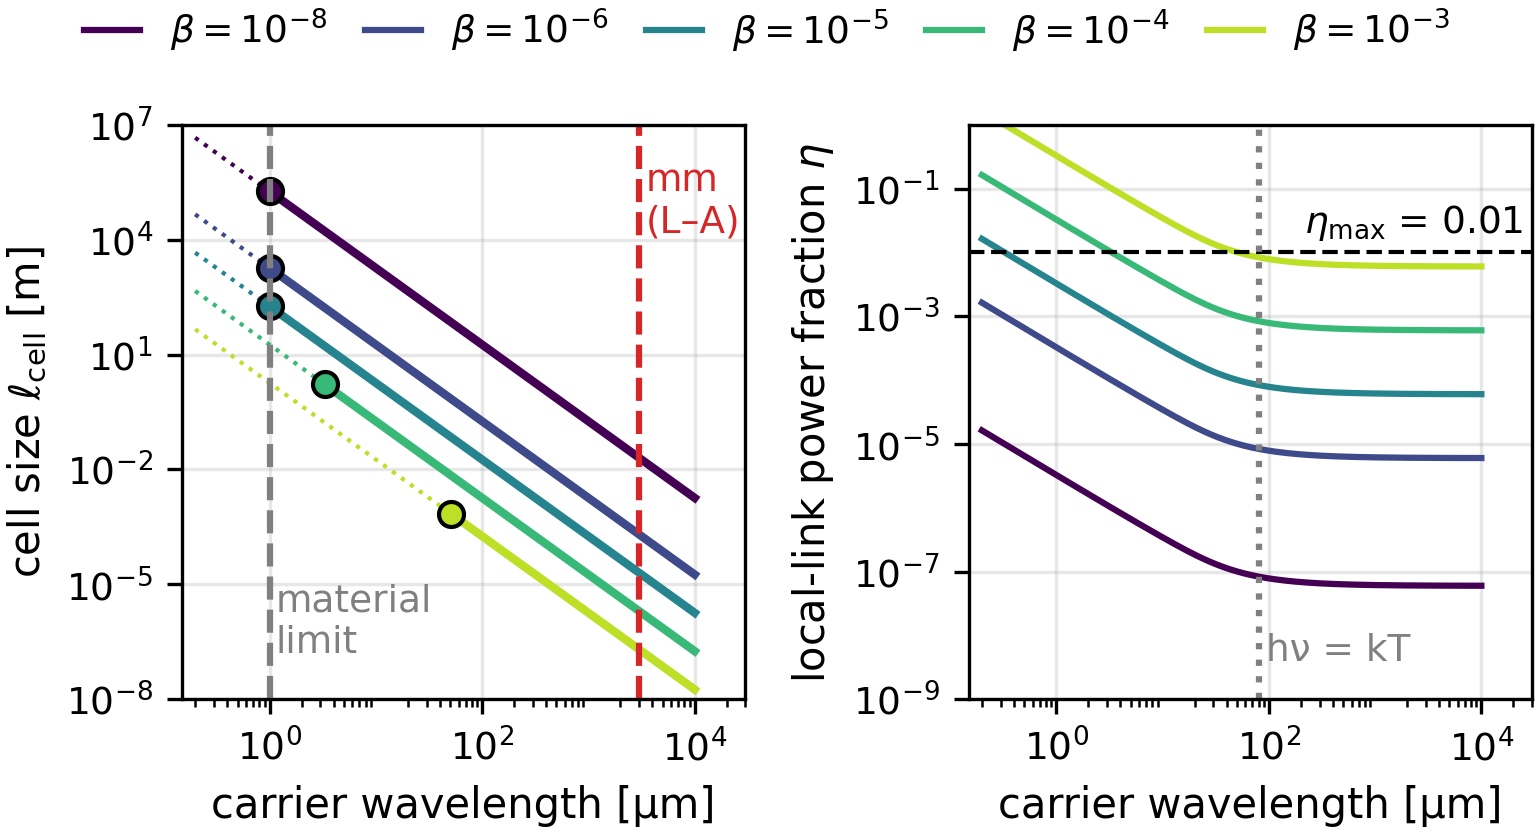
\includegraphics[width=\figwidth]{fig9_carrier_optimum.png}
\caption{Left: size of the bandwidth-balanced cell against carrier wavelength for several bits-per-operation ratios $\beta$. Solid segments are affordable ($\eta\le\eta_{\rm max}$, $\lambda\ge1\,\mu$m), dotted segments are not, and circles mark the optimum; the red line marks the 3\,mm links of Laughlin et al. (L--A). Right: power fraction spent on local links. The cost per bit rises from about $\kTl$ to $h\nu\ln2$ once $h\nu>kT$.}
\label{fig:carrier}
\end{widefigure}

\begin{widetable}
\centering
\caption{Optimal designs (FCC lattice, $\eta_{\rm max}=0.01$, $\tau_{\rm p}=1\,\mu$s, about 10 nodes per cell side). Leakage is the fraction of $L_\ast$ escaping in the communication band (\S\ref{sec:leak}).}
\label{tab:optima}
\small
\fittable{\begin{tabular}{cccccccccc}
\toprule
$\beta$ & $\lambda$ & $\Delta R$ & $d$ & face & $\lcell$ & $1/\tau_{\rm cell}$ & $P_{\rm node}$ & $\eta$ & leak$/L_\ast$ \\
\midrule
$10^{-8}$ & 1\,$\mu$m & 22\,AU$^a$ & 3.7\,km & 6.1\,cm & 180\,km & 1.3\,kHz & 0.63\,W & $3\times10^{-6}$ & $4\times10^{-7}$ \\
$10^{-6}$ & 1\,$\mu$m & 0.052\,AU & 182\,m & 1.3\,cm & 1.8\,km & 51\,kHz & 31\,mW & $3\times10^{-4}$ & $4\times10^{-5}$ \\
$10^{-5}$ & 1\,$\mu$m & $7.8\times10^7$\,m & 18\,m & 4.3\,mm & 180\,m & 78\,kHz & 3\,mW & $3\times10^{-3}$ & $4\times10^{-4}$ \\
$10^{-4}$ & 3.3\,$\mu$m & 1.9\,km & 17\,cm & 0.7\,mm & 1.7\,m & 82\,kHz & 92\,$\mu$W & 0.01 & $1.2\times10^{-3}$ \\
$10^{-3}$ & 51\,$\mu$m & 0.2\,mm$^b$ & 0.2\,mm & 0.1\,mm & 0.7\,mm & 250\,kHz & 1.9\,$\mu$W & 0.01 & $1.2\times10^{-3}$ \\
\bottomrule
\multicolumn{10}{l}{\footnotesize $^a$capped at $0.1R$; $^b$single node layer (a monolithic ``fabric'').}
\end{tabular}}
\end{widetable}

Table~\ref{tab:optima} lists the optima. For the fiducial $\beta=10^{-6}$ the cloud uses $1\,\mu$m links between rhombic-dodecahedral nodes with faces about 1.3\,cm across, spaced 182\,m apart. The nodes fill a shell 0.052\,AU thick in about $4\times10^{7}$ layers. Each node dissipates 31\,mW, performs $1.8\times10^{19}$ bit operations per second, and drives twelve $3\times10^{13}$\,bit\,s$^{-1}$ links. A cell is 1.8\,km across and contains about 1400 nodes. Signals relay at $0.38c$, so a cell is crossed in $20\,\mu$s and processes about 0.8\,mJ per crossing. The whole cloud comprises about $1.8\times10^{28}$ such cells. Figure~\ref{fig:volume} shows one cell, its lattice and a single node at increasing magnification, and Fig.~\ref{fig:ladder} places every scale on one diagram. As $\beta$ rises the optimum moves to longer wavelengths and thinner shells. By $\beta=10^{-3}$ the energy limit pushes the carrier to the far infrared and the structure collapses to a single sheet of sub-millimeter nodes, the astrophysical analog of a wafer-scale two-dimensional mesh.

\begin{widefigure}
\centering
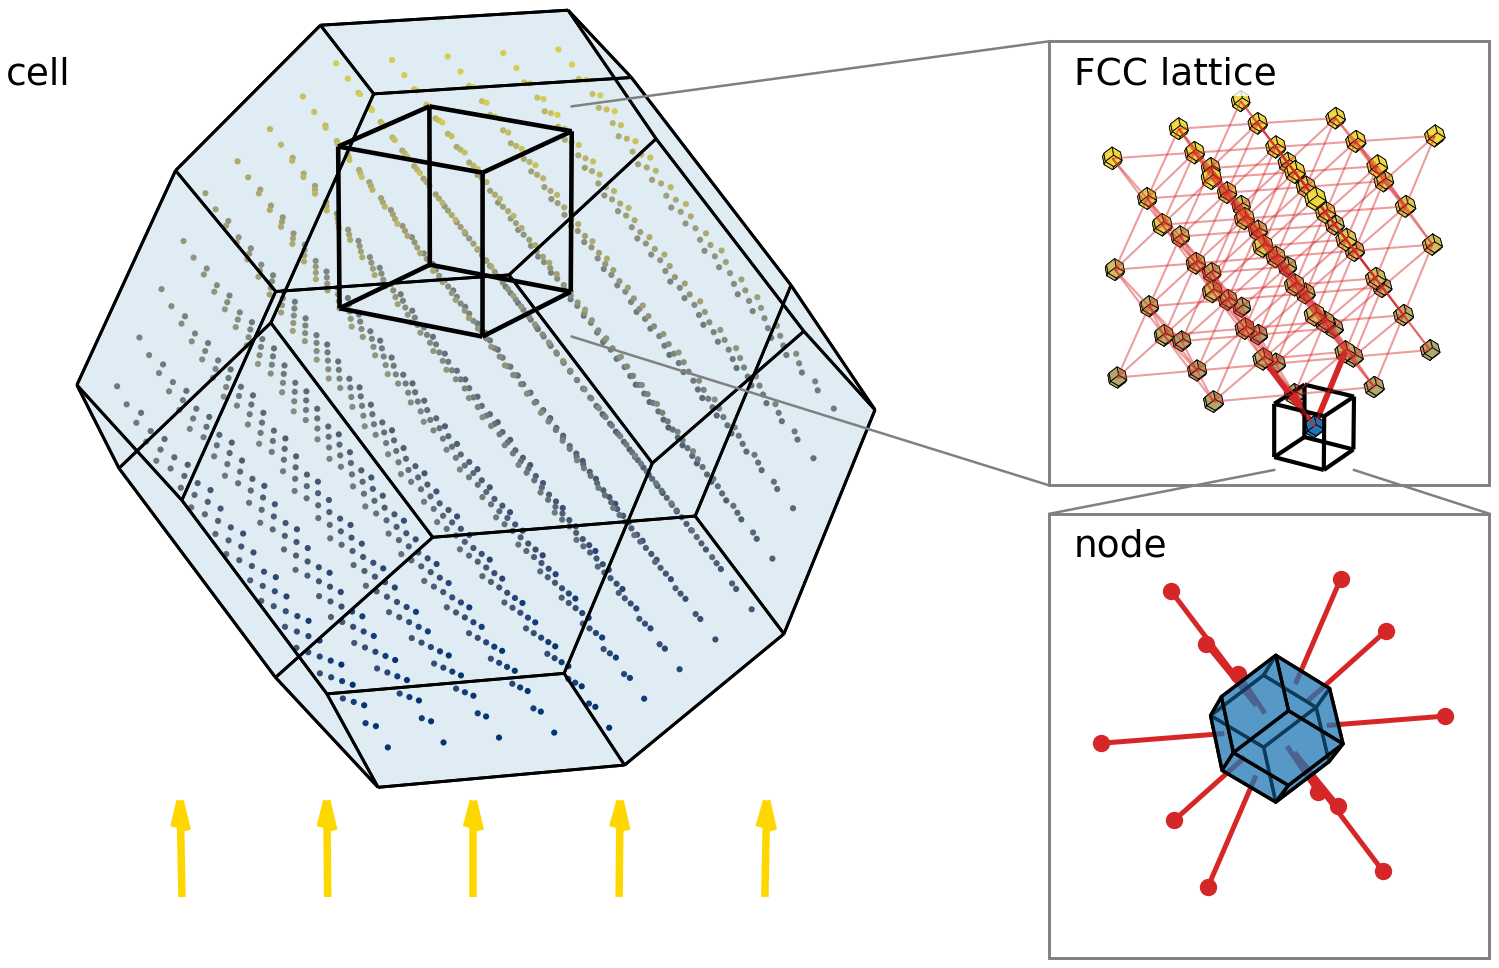
\includegraphics[width=\figwidth]{fig11_local_volume.png}
\caption{One cell of the optimal ($\beta=10^{-6}$) cloud, zooming into its node lattice and one node. Left: the cell as a truncated octahedron (Kelvin's cell; \S\ref{sec:cells}), holding about 1400 nodes (dots, colored by radial depth) in the volume of a 1.8\,km cube; its square faces, 2.3\,km apart, face the star (yellow arrows). Top right: the boxed patch of the FCC lattice, nodes 182\,m apart (greatly enlarged) linked to their nearest neighbors (red). Bottom right: the highlighted node, a rhombic dodecahedron whose 12 faces, each about 1.3\,cm across, are Fresnel-matched apertures pointing at its neighbors.}
\label{fig:volume}
\end{widefigure}

\begin{colfigure}
\centering
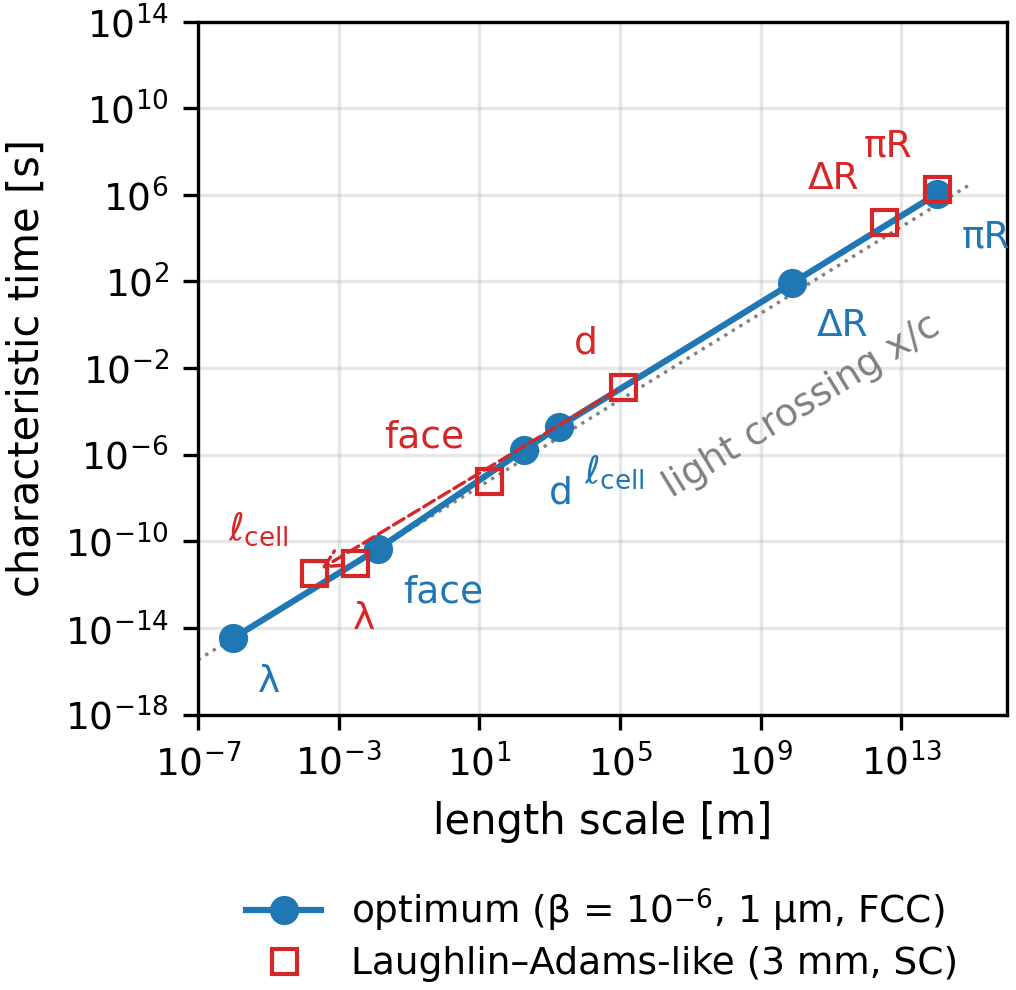
\includegraphics[width=\colfigwidth]{fig10_scale_ladder.png}
\caption{Hierarchy of computing scales and their characteristic times for the optimal design (blue) and a Laughlin--Adams-like 3\,mm design (red): carrier wavelength $\lambda$, node face, hop length $d$, cell size $\lcell$, shell thickness $\Delta R$ and half circumference $\pi R$. The dashed arrow runs from the millimeter design's hop length to its cell size: its bandwidth-balanced cell (about 0.2\,mm) is smaller than its own 19\,m nodes, let alone the 120\,km node spacing, so that design is bandwidth-starved.}
\label{fig:ladder}
\end{colfigure}

\subsection{Computing power of a cell}\label{sec:cellpower}
A cell's throughput is the absorbed power that it contains, {\relpenalty=200 $P_{\rm cell}=F\lcell^3/\Delta R$}, divided by $\kTl$. With about 10 nodes across, the optimal cells for $\beta=10^{-6}$--$10^{-4}$ hold about 1400 nodes, so $P_{\rm cell}\approx1400\,P_{\rm node}$, from 43\,W down to 0.13\,W. At $\beta=10^{-8}$ the thickness cap leaves 49 nodes across a cell, which then draws 100\,kW. Table~\ref{tab:earth} compares them with terrestrial machines.

Converting floating-point operations into irreversible bit operations requires an assumed factor, which we take as $3\times10^4$ bit operations per double-precision operation (range $10^4$--$10^5$, as in the estimate of $\beta$). Every ``FLOPS-equivalent'' figure below scales linearly with that factor. The fiducial cell then performs $2.5\times10^{22}$ bit operations per second, or about 0.85\,EFLOPS-equivalent. That is roughly half of El Capitan, which runs the HPL benchmark at 1.81\,EFLOPS on 29.7\,MW \citep{TOP5002026}. The cell does it on 43\,W, the power of an incandescent light bulb, spread over 1400 centimeter-sized nodes in a cube 1.8\,km on a side. A single 31\,mW node matches about $6\times10^{14}$\,FLOPS-equivalent, about 1/700 of Fugaku.

\begin{widetable}
\centering
\caption{A Black Cloud cell compared with terrestrial computers. Terrestrial throughput is HPL $R_{\rm max}$ with the listed power \citep{TOP5002026}. Bit operations assume $3\times10^4$ per floating-point operation. The mining-ASIC efficiency is from \citet{LaughlinAdams2021}. The last column is the energy per bit operation in units of $\kTl$ at the machine's own temperature (300\,K for terrestrial hardware); the cloud is assumed to run at the Landauer limit.}
\label{tab:earth}
\fittable{%
\begin{tabular}{lcccccc}
\toprule
Machine & Size & Power & Bit ops s$^{-1}$ & FLOPS-equiv. & Bit ops J$^{-1}$ & $E/\kTl$ \\
\midrule
Cloud node ($\beta=10^{-6}$) & 1.3\,cm faces & 31\,mW & $1.8\times10^{19}$ & $6\times10^{14}$ & $5.9\times10^{20}$ & 1 \\
Cloud cell ($\beta=10^{-5}$) & 180\,m & 4.3\,W & $2.5\times10^{21}$ & $8.5\times10^{16}$ & $5.9\times10^{20}$ & 1 \\
Cloud cell ($\beta=10^{-6}$) & 1.8\,km & 43\,W & $2.5\times10^{22}$ & $8.5\times10^{17}$ & $5.9\times10^{20}$ & 1 \\
Cloud cell ($\beta=10^{-8}$) & 180\,km & 100\,kW & $6.0\times10^{25}$ & $2.0\times10^{21}$ & $5.9\times10^{20}$ & 1 \\
\midrule
Fugaku & building & 29.9\,MW & $1.3\times10^{22}$ & $4.4\times10^{17}$ & $4.4\times10^{14}$ & $8\times10^{5}$ \\
El Capitan & building & 29.7\,MW & $5.4\times10^{22}$ & $1.8\times10^{18}$ & $1.8\times10^{15}$ & $2\times10^{5}$ \\
LineShine & building & 42.2\,MW & $6.6\times10^{22}$ & $2.2\times10^{18}$ & $1.6\times10^{15}$ & $2\times10^{5}$ \\
SHA-256 mining ASIC & board & -- & -- & -- & $2\times10^{13}$ & $2\times10^{7}$ \\
\midrule
Whole Black Cloud & 220\,AU & $7.6\times10^{29}$\,W & $4.5\times10^{50}$ & $1.5\times10^{46}$ & $5.9\times10^{20}$ & 1 \\
\bottomrule
\end{tabular}}
\end{widetable}

Almost all of the factor of $3\times10^5$ in energy efficiency comes from where present hardware sits relative to the Landauer bound: El Capitan spends about $2\times10^5\,\kTl$ (at 300\,K) per bit operation. Only a factor of 1.7 comes from running at 177\,K rather than room temperature. The comparison therefore measures the headroom that \citet{LaughlinAdams2021} assume that a mature technology will close, not a capability that the model demonstrates.

In time, by contrast, a cell resembles a terrestrial machine. Its clock runs at about 50\,kHz, set by about 12 relay hops of $1.6\,\mu$s each. A hop on Fugaku's Tofu-D network takes 0.49\,$\mu$s \citep{Ajima2018}, and a global reduction across Fugaku about $9\,\mu$s (\S\ref{sec:cloud}), comparable to the $20\,\mu$s cell crossing. The sharp contrast is in mass. The fiducial cell has a mass of only 0.34\,g, the cloud's mass divided among its $1.8\times10^{28}$ cells. In Laughlin's ``oklo'' unit of computational intensity, one bit operation per gram per second \citep{Laughlin2014}, the cell runs at $7.5\times10^{22}$\,oklo, against 50\,oklo that Laughlin estimated for Earth from the DNA copying of its biosphere \citep{Laughlin2014,LaughlinAdams2021} and about $10^{12}$\,oklo for a current smartphone \citep{Laughlin2021blog}. The whole cloud is equivalent to about $8\times10^{27}$ El Capitans. It reaches that figure not by building faster machines but by tiling $10^{28}$ gram-scale, kilometer-sized cells, each roughly as capable as the largest computers on Earth.

\subsection{Bandwidth of the millimeter design}\label{sec:submm}
We apply the same accounting to the original proposal. \citet{LaughlinAdams2021} allowed carriers between 1\,mm and 1\,cm and adopted 3\,mm, which we use here. With $\Delta R=0.1R$ and a simple cubic lattice, this gives nodes about 19\,m across, spaced 120\,km apart, each dissipating 31\,kW. Each node performs $1.8\times10^{25}$ bit operations per second but has only $6\times10^{10}$\,bit\,s$^{-1}$ of links. That ratio, $3\times10^{-15}$, is $3\times10^{8}$--$3\times10^{9}$ times below a terrestrial supercomputer's. Equivalently, Eq.~\eqref{eq:lcell} gives $\lcell\approx0.2$\,mm, $6\times10^{8}$ times smaller than the node spacing. Even at 1\,mm, the short end of their range, the cell would be only 2\,mm across, since $\lcell\propto\lambda^{-2}$. Globally, the bisection bandwidth of a great-circle cut is $2\pi R\,\tau f_B c/\lambda^2$, again independent of $\Delta R$. This is $7\times10^{26}$\,bit\,s$^{-1}$ at 3\,mm and $6\times10^{33}$\,bit\,s$^{-1}$ at $1\,\mu$m, compared with $4.5\times10^{50}$ bit operations per second of computing. The total of $7\times10^{42}$\,bit\,s$^{-1}$ that \citet{LaughlinAdams2021} found counts channels over the whole surface of the shell, so it bounds the traffic that can cross that surface. Traffic between the two halves of the shell is limited by the bisection instead, which at 3\,mm is about $10^{16}$ times smaller. Any Black Cloud is therefore an archipelago of independent cells. Long backbone links (\S\ref{sec:prop}) shorten latencies but cannot increase bandwidth, since a pair of hubs across the cavity shares at most one spatial mode.

%======================================================================
\section{Workloads across the computing hierarchy}\label{sec:workloads}
%======================================================================

The hierarchy of \S\ref{sec:cells} sorts algorithms by two numbers. The first is the bandwidth they need per operation, which sets the largest level whose links can feed them. The second is how often they must synchronize, which sets how much work fits between barriers. Table~\ref{tab:workloads} lists both for the node, the cell and the whole cloud of the fiducial ($\beta=10^{-6}$) design. The governing rule is the one behind Rent's rule \citep{Landman1971,Christie2000}. An algorithm whose communication grows only as the surface of its domain (local coupling) can be scaled to any level by enlarging each processor's share. An algorithm whose communication grows as its volume (global coupling) is confined to the level whose bandwidth per operation it fits.

\begin{widetable}
\centering
\caption{Computing resources at each level of the fiducial design ($\beta=10^{-6}$, $\lambda=1\,\mu$m, FCC). ``Sync'' is the time for one round of communication at that level: a neighbor hop for a node, a cell crossing for a cell, and one global superstep (gather and broadcast) over a backbone of 24 hubs, or over the mesh alone in parentheses, for the cloud.}
\label{tab:workloads}
\fittable{%
\begin{tabular}{lccccccl}
\toprule
Level & Power & Bit ops s$^{-1}$ & Bits per op & Sync & Ops per sync & Count & Natural workloads \\
\midrule
Node & 31\,mW & $1.8\times10^{19}$ & $2\times10^{-5}$ & 1.6\,$\mu$s & $2.9\times10^{13}$ & $2.5\times10^{31}$ & dense kernels, search, sampling \\
Cell & 43\,W & $2.5\times10^{22}$ & $10^{-6}$ & 20\,$\mu$s & $5\times10^{17}$ & $1.8\times10^{28}$ & stencils, linear algebra, models \\
Cloud & $7.6\times10^{29}$\,W & $4.5\times10^{50}$ & $1.4\times10^{-17}$ & 9.4\,d (26\,d) & $4\times10^{56}$ & 1 & ensembles, evolution, reductions \\
\bottomrule
\end{tabular}}
\end{widetable}

\subsection{Node-level computation}
A node is a 31\,mW rhombic dodecahedron that performs $1.8\times10^{19}$ bit operations per second, about $6\times10^{14}$\,FLOPS-equivalent. Its twelve links together carry $3.6\times10^{14}$\,bit\,s$^{-1}$, or $2\times10^{-5}$ bits per operation, so a node-level kernel must perform about $5\times10^4$ bit operations for every bit it exchanges. Dense linear algebra reaches this intensity because a block of side $n$ costs $\sim n^3$ operations for $\sim n^2$ words of data. A matrix-multiply block of side $n\gtrsim300$ held within one node (64-bit words, $3\times10^4$ bit operations per multiply--add) stays within the bandwidth of the node's links, and communication-avoiding formulations extend this to factorizations and eigenproblems \citep{Ballard2011}. Monte Carlo sampling, brute-force search over candidate keys or proofs, and inference with model weights stored on the node need almost no communication and run at full node speed.

Nodes also carry the machine's housekeeping: pointing twelve beams at neighbors that drift with the outflow, correcting bit errors, modulating radiating area in a thermostatted design, and rebuilding their neighborhood. All of these are local control loops whose communication stays within a few hops.

\subsection{Cell-level computation}
A cell of about 1400 nodes draws 43\,W, performs $2.5\times10^{22}$ bit operations per second and is crossed in $20\,\mu$s. Its bisection bandwidth is $1.3\times10^{16}$\,bit\,s$^{-1}$, which by construction supplies $\beta=10^{-6}$ bits per operation. This is the level for tightly coupled parallel algorithms of the kind that run on terrestrial supercomputers.

A three-dimensional stencil illustrates the scaling. Stencils are the kernel of cellular automata and of explicit solvers for partial differential equations. Take 64 bits exchanged per halo point and $3\times10^5$ bit operations (about 10 floating-point operations) per point update. A node's links would be fed by a subdomain only 64 points on a side, but each step must then wait for a neighbor hop of $1.6\,\mu$s. The subdomain that makes computation outlast that latency is $458^3\approx10^8$ points. Each node then updates its subdomain every $1.6\,\mu$s ($6\times10^5$ steps per second) while its halo exchange takes $0.22\,\mu$s. The stencil is limited by latency, not bandwidth. Because a stencil's communication grows only as its surface, it is not confined to a cell. The whole cloud can run a single stencil of $2.4\times10^{39}$ points. An explicit scheme moves information at most one point per step, however, so a signal in the simulated domain travels at about 250\,km\,s$^{-1}$, three orders of magnitude slower than the machine's own relays, and takes 13\,yr to cross the shell.

Hierarchical $N$-body methods such as the fast multipole method \citep{Greengard1987} split naturally along the hierarchy: near-field interactions are local, while the coarse levels of the tree require reductions across cells and become latency-bound above the cell scale. Fast Fourier transforms and other all-to-all exchanges move a cell's whole dataset across its bisection at every transpose, so they are best confined to nodes or single cells. Dense attention in neural networks is one such exchange. Large neural networks can be split by model across the nodes of a cell and trained in parallel across cells with infrequent parameter averaging, the federated-averaging strategy designed for slow links \citep{McMahan2016}.

\subsection{Cloud-level computation}\label{sec:cloud}
The cloud as a whole is a bulk-synchronous parallel machine \citep{Valiant1990}. A global superstep consists of a gather to a reduction root and a broadcast from it. It takes 9.4\,d over the backbone of 24 hubs used in \S\ref{sec:prop} and 26\,d over the mesh alone. Each leg crosses the cavity between hubs at the speed of light, but must still cross up to $32^\circ$ of mesh between a hub and the farthest cell it serves. A backbone dense enough to remove that mesh leg would reach the light-crossing bound of 5.3\,d: twice $2R/c$, plus an hour of processing at each hub on the way. Between barriers the cloud performs $4\times10^{56}$ bit operations but can exchange at most $5\times10^{39}$ bits across its bisection, about $2.8\times10^{11}$ bits (36\,GB) per cell. Over a $10^4$\,yr pre-planetary-nebula lifetime of the host \citep{Laughlin2021blog,Gilster2021} this allows $4\times10^5$ supersteps ($1.4\times10^5$ over the mesh), and about $1.2\times10^4$ within one 300\,yr rebuilding cycle \citep{LaughlinAdams2021}. The lifetime total is $1.4\times10^{62}$ bit operations, consistent with the order-$10^{62}$ estimate of \citet{Laughlin2021grab}.

The binding constraint at this level is depth, not throughput. On Fugaku a binary reduction tree over 158{,}976 nodes \citep{RIKEN2021} has 18 levels, so at the 0.49\,$\mu$s Tofu-D hop latency \citep{Ajima2018} one global reduction takes about $9\,\mu$s. Fugaku therefore performs as many globally synchronized steps in a few seconds as a Black Cloud does in its lifetime. This is the quantitative form of the conclusion of \citet{LaughlinAdams2021} that a Black Cloud must be massively parallel. Whole-star computations are therefore those with enormous width and shallow global depth:
\begin{itemize}
\item \emph{Ensembles and exhaustive search.} At $10^4$ bit operations per trial, comparable to one floating-point multiply--add (\S\ref{sec:beta}), the lifetime budget is enough to search a space of about $2^{193}$ candidates. Merely counting through $2^{256}$ states at the Landauer limit would cost $2\times10^{56}$\,J, fifteen orders of magnitude more than the $2.4\times10^{41}$\,J the star supplies over the AGB phase.
\item \emph{Evolutionary computation.} The $1.8\times10^{28}$ cells form a natural island model: each evolves a population locally and exchanges its best members at every superstep.
\item \emph{Map and reduce.} Statistics, model averages and search results flow up a reduction tree once per superstep, in the pattern of MapReduce \citep{Dean2008}.
\item \emph{Global iterative solvers.} Krylov methods need a global inner product every iteration, so they are limited to a few times $10^5$ iterations over the cloud's lifetime and must be preconditioned to converge within that budget.
\item \emph{Self-maintenance.} Coordinating the rebuild of the structure, its thermal regulation and the allocation of work across cells needs only a few global decisions per rebuild cycle, comfortably within the $10^4$ supersteps available.
\end{itemize}

\subsection{Observable consequences of the workload mix}
Light-travel smoothing (\S\ref{sec:filter}) acts very differently on the three levels. A cell's 50\,kHz clock is suppressed to about $10^{-11}$ before incoherent averaging over $10^{28}$ cells, so node- and cell-level activity is invisible in unresolved data. A global superstep cannot be shorter than twice the light-crossing time, so its cadence always survives: 88\% of the amplitude remains for a 9.4\,d backbone superstep (66\% at the 5.3\,d bound) and 98\% for a 26\,d mesh superstep. Whole-star algorithms with synchronized exchange phases would therefore modulate the communication band with a period of days to weeks, slower than any internal clock and faster than the Mira cycle. Whether they do depends on scheduling (\S\ref{sec:incoherent}).

%======================================================================
\section{Results}\label{sec:results}
%======================================================================

\subsection{Signal propagation across the shell}\label{sec:prop}

For the millimeter design, with 20\,m node apertures close to the 19\,m nodes of \S\ref{sec:submm}, we simulate propagation on a coarse-grained shell: 6000 cells on a jittered Fibonacci lattice, each linked to its 8 nearest neighbors, with arrival times computed by Dijkstra's algorithm. The energy-optimal hop is the Fresnel distance $A/\lambda=130$\,km, giving a relay speed of $0.31c$ for $\tau_{\rm p}=1$\,ms. A broadcast takes 13\,d to reach the antipode (Fig.~\ref{fig:links} and Fig.~\ref{fig:maps}, left). Adding 24 hubs with 10\,km apertures that beam across the cavity cuts the worst-case arrival time to 6.6\,d (Fig.~\ref{fig:maps}, right) and the energy per long-haul bit from $2\times10^9$ to $8\times10^6\,\kTl$. The hubs sit at the vertices of a snub cube, the best-separated arrangement of 24 points on a sphere \citep{Robinson1961}, so no point of the shell lies more than $32^\circ$ from a hub. The same 24 hubs scattered at random leave cells up to $54^\circ$ from the nearest hub, and the worst case rises to 7.8\,d. The optimal near-infrared design relays faster ($0.38c$), but its global synchronization still takes days (\S\ref{sec:cloud}).

\begin{colfigure}
\centering
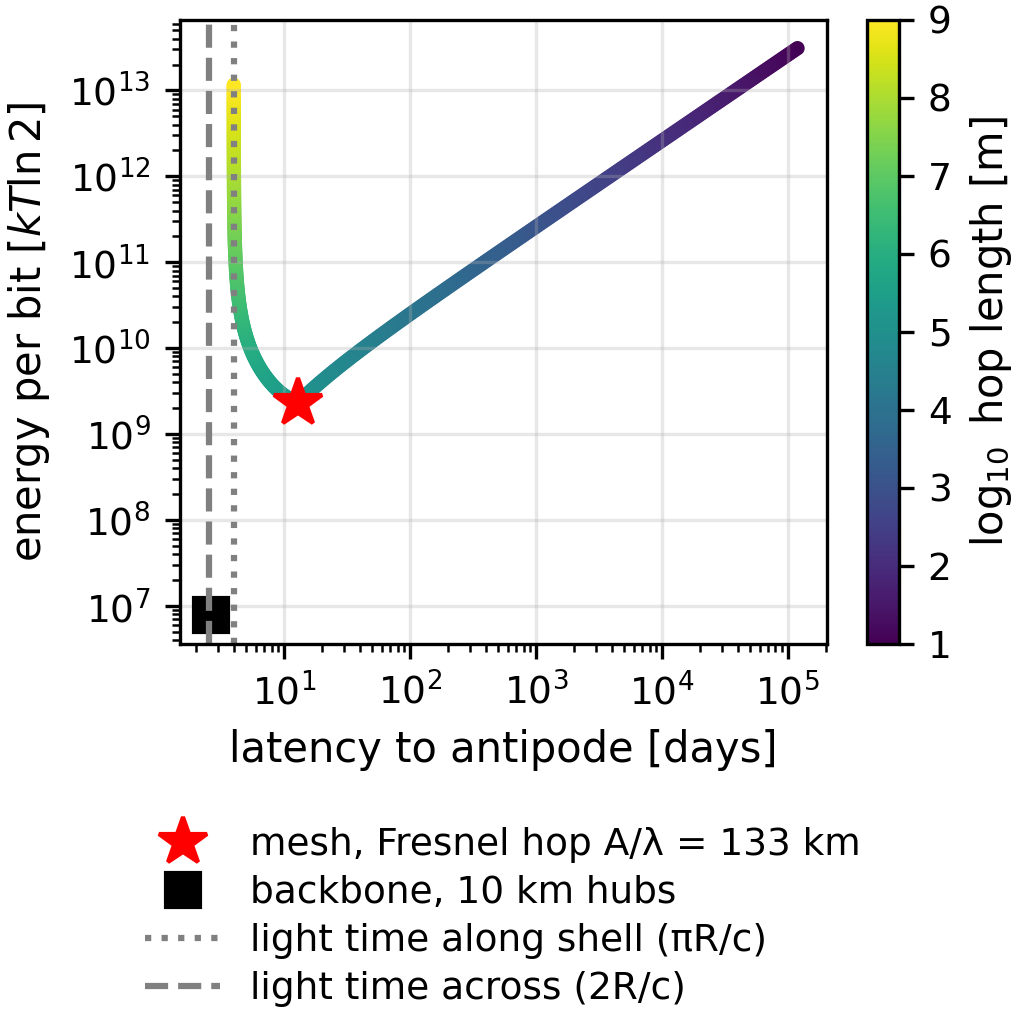
\includegraphics[width=\colfigwidth]{fig3_link_economics.png}
\caption{Energy per bit against latency for moving one bit to the antipode ($D=\pi R$) in the millimeter design, as a function of mesh hop length (color). The red star marks the Fresnel hop $A/\lambda=130$\,km; the black square marks a direct link between 10\,km backbone hubs.}
\label{fig:links}
\end{colfigure}

\begin{widefigure}
\centering
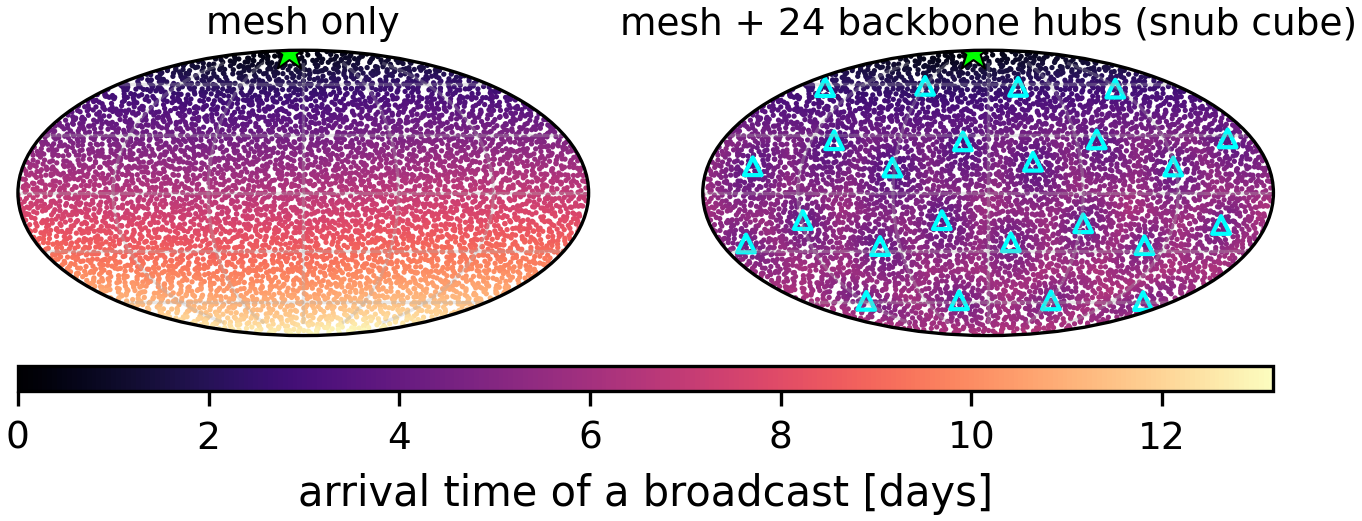
\includegraphics[width=\figwidth]{fig4_propagation.png}
\caption{Arrival time of one broadcast across the shell of the millimeter design, for the mesh alone (left) and the mesh plus 24 backbone hubs at the vertices of a snub cube (right, cyan triangles), on one color scale. Each map is a Mollweide (equal-area) projection of the whole shell at $R=220$\,AU, plotting the longitude and latitude of each cell's direction as seen from the star, measured about the model's arbitrary polar axis. The graticule is every $60^\circ$ in longitude and $30^\circ$ in latitude, the star lies at the center of the sphere behind the map, and each dot is one of the 6000 coarse-grained cells. The broadcast starts at the green star, near the north pole ($86^\circ$ latitude), so arrival time grows toward the south.}
\label{fig:maps}
\end{widefigure}

\subsection{Thermal emission and the workload}\label{sec:thermal}
Every joule of absorbed starlight is re-radiated within $\tau_{\rm th}\le0.36$\,s whether nodes compute or idle, so the bolometric light curve is set entirely by the star and the geometry. Nor can a thermal store hide the stellar pulsation: flattening one half-cycle means absorbing the excess $\delta L\,L_\ast P_{\rm Mira}/\pi=3.4\times10^{36}$\,J, which would heat an Earth mass of carbon by at least $2.7\times10^8$\,K.

\subsection{Spectral shape}

\begin{colfigure}
\centering
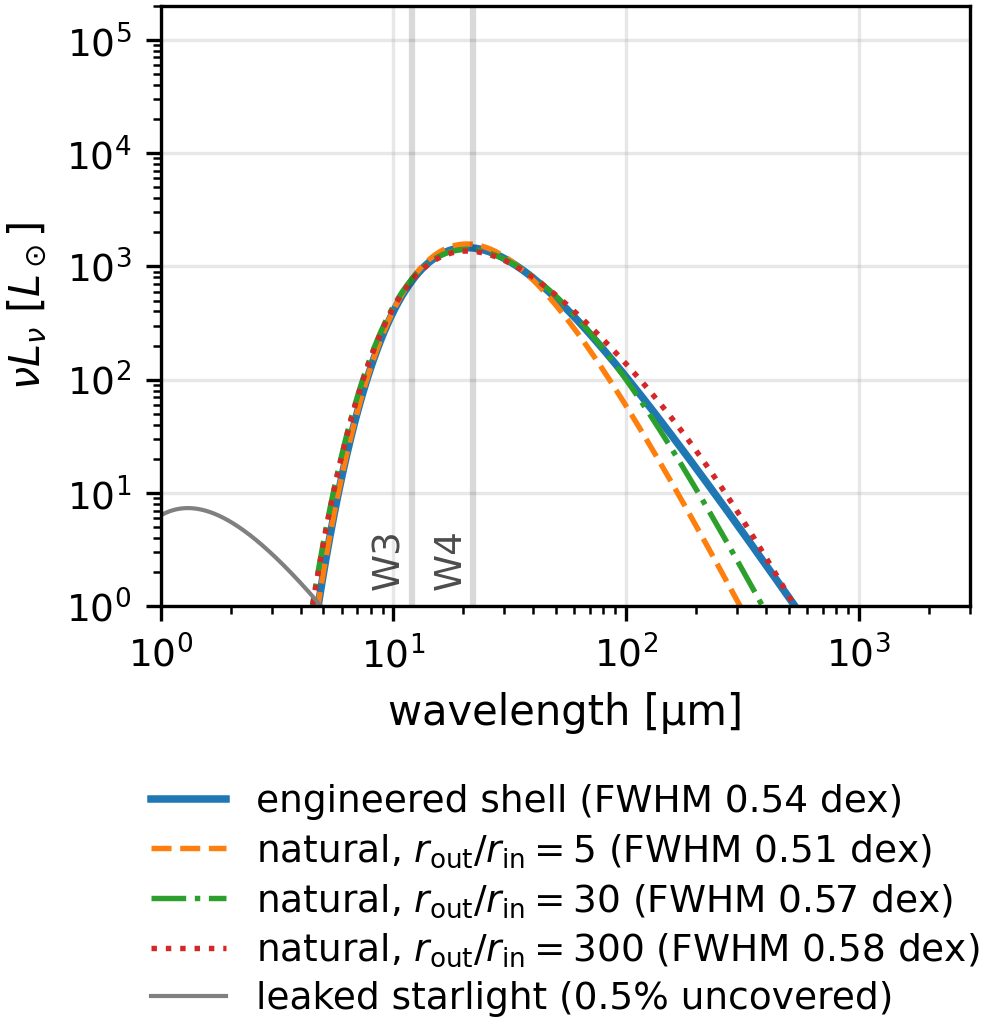
\includegraphics[width=\colfigwidth]{fig1_sed.png}
\caption{Spectral energy distributions at equal infrared luminosity. Solid: engineered single-temperature shell. Broken: optically thin natural envelopes ($n\propto r^{-2}$, $\kappa_\nu\propto\nu$) with peaks matched to the shell. Gray: starlight leaking through the 0.5\% uncovered fraction.}
\label{fig:sed}
\end{colfigure}

We compare the engineered shell with optically thin natural envelopes ($n\propto r^{-2}$, $\kappa_\nu\propto\nu^\beta$, $T_d\propto r^{-2/(4+\beta)}$). We take $\beta=1$, consistent with the submillimeter emissivity index slightly below 1 measured for both carbon- and oxygen-rich evolved-star envelopes \citep{Knapp1993}, with inner temperatures chosen to match the peak of $\nu L_\nu$. The temperature gradient broadens the natural SED, but the emissivity narrows it again, and the two effects nearly cancel. Natural envelopes have mid-infrared widths of 0.51--0.58\,dex against 0.54\,dex for a blackbody (Fig.~\ref{fig:sed}). The ``unnaturally clean blackbody'' criterion therefore has little power at mid-infrared wavelengths. The long-wavelength slope survives: $\alpha_{450/850\,\mu{\rm m}}\approx1.9$ for a gray shell against 2.6--2.9 for dust. This assumes that the structure is engineered to be gray in the sub-mm.

\subsection{Infrared variability across the Mira cycle}

\begin{widefigure}
\centering
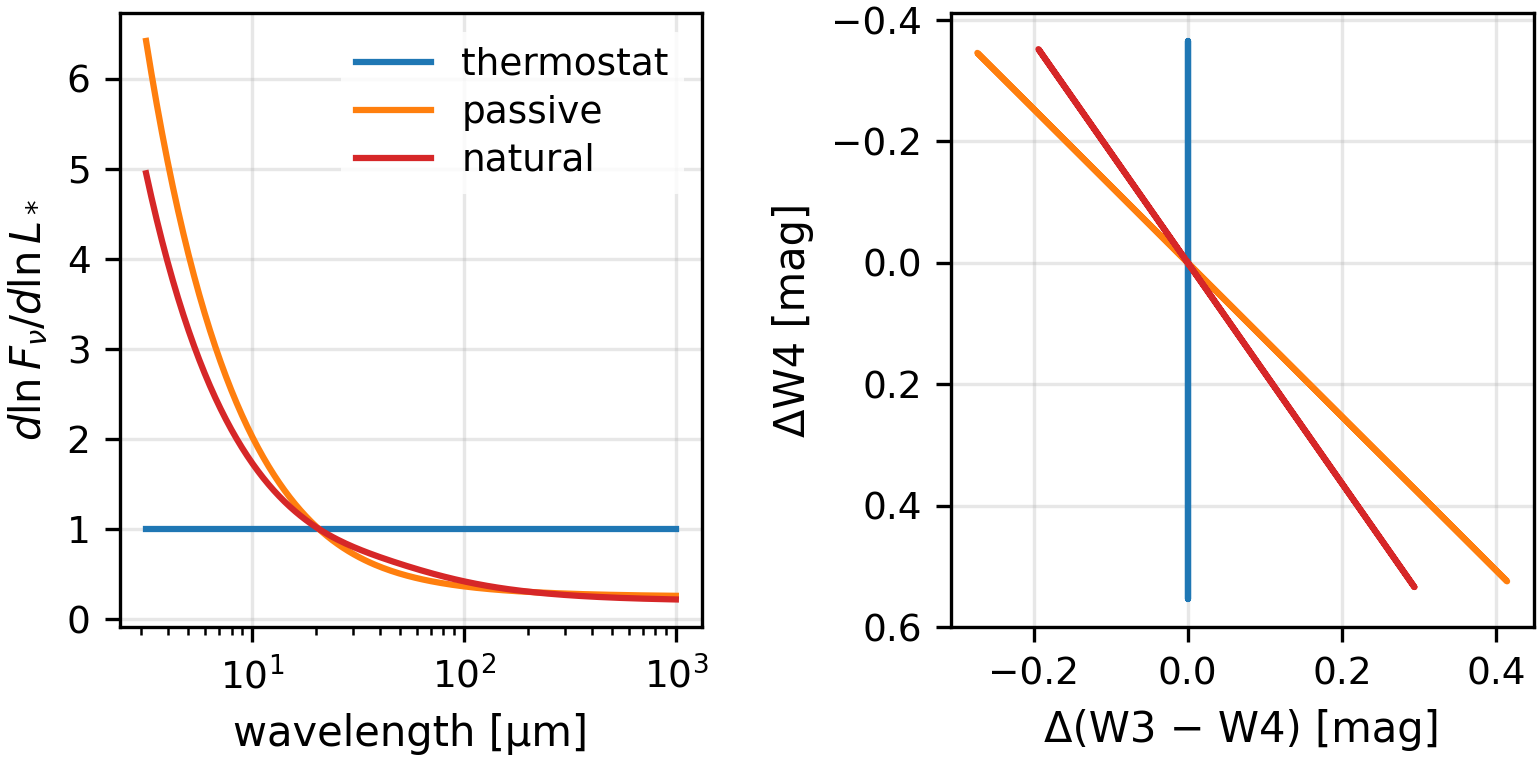
\includegraphics[width=\figwidth]{fig2_mira_response.png}
\caption{Left: logarithmic response of $F_\nu$ to stellar luminosity for a thermostatted shell, a passive shell and a natural envelope. Right: the resulting W4 versus W3$-$W4 track over a $\pm40\%$ Mira cycle.}
\label{fig:mira}
\end{widefigure}

A passive shell ($T\propto L_\ast^{1/4}$) and a natural envelope respond almost identically to the stellar pulsation (Fig.~\ref{fig:mira}). The response $d\ln F_\nu/d\ln L_\ast$ is 1.69 and 1.49 at 12\,$\mu$m and 0.95 and 0.96 at 22\,$\mu$m. Only a thermostatted shell varies achromatically, because it holds $T$ fixed and modulates its radiating area. Its W3$-$W4 color stays fixed while W4 swings by about $\pm0.4$\,mag. Color-invariant mid-infrared variability of a Mira host is a sufficient technosignature, not a necessary one.

\subsection{Communication-band leakage}\label{sec:leak}

\begin{widefigure}
\centering
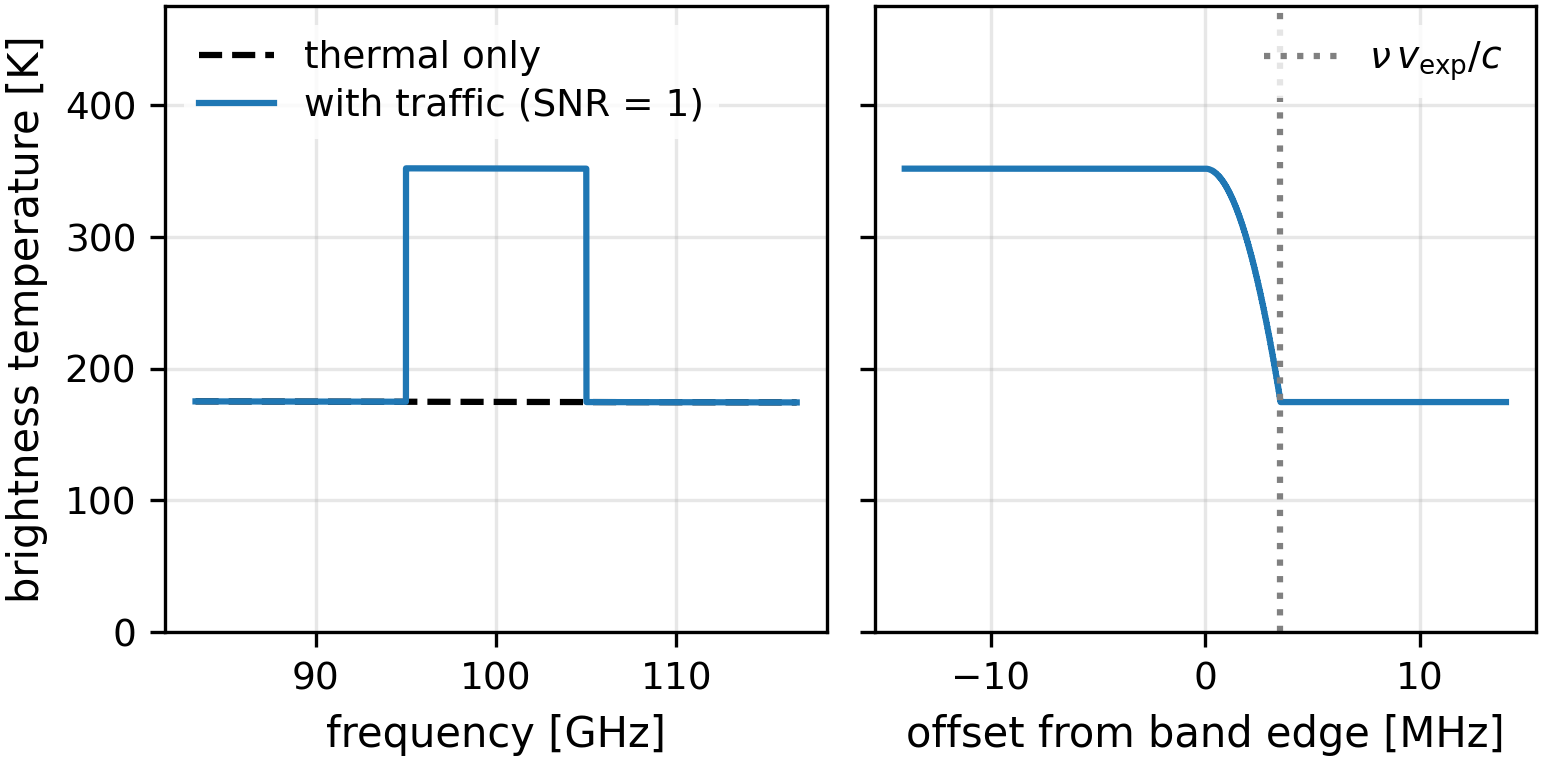
\includegraphics[width=\figwidth]{fig7_comm_band.png}
\caption{Millimeter case. Left: brightness temperature around the communication band, for the thermal surface alone (dashed) and including traffic leakage at a per-mode SNR of 1. Right: the upper band edge, smeared over $\nu_{\rm c}v_{\rm exp}/c\approx3.5$\,MHz by the outflow.}
\label{fig:band}
\end{widefigure}

\emph{Millimeter links.} If the shell is optically thick in band and its links run at per-mode SNR $\approx1$, the outermost layer radiates its traffic at brightness temperature $\approx2T$. The escaping power is
\begin{equation}
P_{\rm leak}=4\pi R^2\,\pi\,\frac{2k\nu_{\rm c}^2}{c^2}\,{\rm SNR}\,T\,B=2.3\times10^{23}\,{\rm W}.
\end{equation}
Across 10\,GHz this equals the thermal continuum: about 0.19\,Jy at 1\,kpc and 3\,mJy at 8\,kpc. The band appears as a flat-topped plateau with near-vertical edges (Fig.~\ref{fig:band}). Only the approaching hemisphere is visible, with line-of-sight speeds distributed as $p(v)\propto v$ on $[0,v_{\rm exp}]$, so the edges are blueshifted and smeared by about 3.5\,MHz. Well-compressed traffic is statistically thermal, so the signature lies in the band's shape rather than its content.

\emph{Optimal near-infrared links.} For the optimal designs, leakage comes from diffraction spill of local links. Two facing square apertures at Fresnel number $N_F=A/\lambda d$ form a separable problem whose coupling per axis is the largest prolate-spheroidal eigenvalue $\lambda_0(c)$ with $c=\pi N_F/2$ \citep{Slepian1961}. For the Fresnel-matched links of \S\ref{sec:cells} ($N_F=1$) the receiver captures $\lambda_0(\pi/2)^2=0.61$ of the transmitted power, and the remaining 39\% spills past it. The spill escapes through a covering of $\tau=1$. With sources spread uniformly in optical depth, the escape fraction is $(1-e^{-\tau})/2\tau$. The leaked fraction of $L_\ast$ is $4\times10^{-5}$ for $\beta=10^{-6}$, rising to $1.2\times10^{-3}$ for $\beta\ge10^{-4}$ (Table~\ref{tab:optima}). At $1\,\mu$m the 177\,K continuum is negligible. The relevant background is starlight escaping through the uncovered fraction, whose spectrum peaks at $1.03\,\mu$m for $T_\ast=2800$\,K (Wien's law). For the fiducial design the communication band adds about 12\% to the escaping starlight in a 10\% band (8.5\,mJy against 68\,mJy at 1\,kpc). This is a weak but sharply bounded spectral feature on the spectrum of the escaping starlight, from an otherwise cold infrared source. Efficient designs thus hide their traffic in the one part of the spectrum that the star already fills.

\subsection{Light-travel filtering}\label{sec:filter}

\begin{widefigure}
\centering
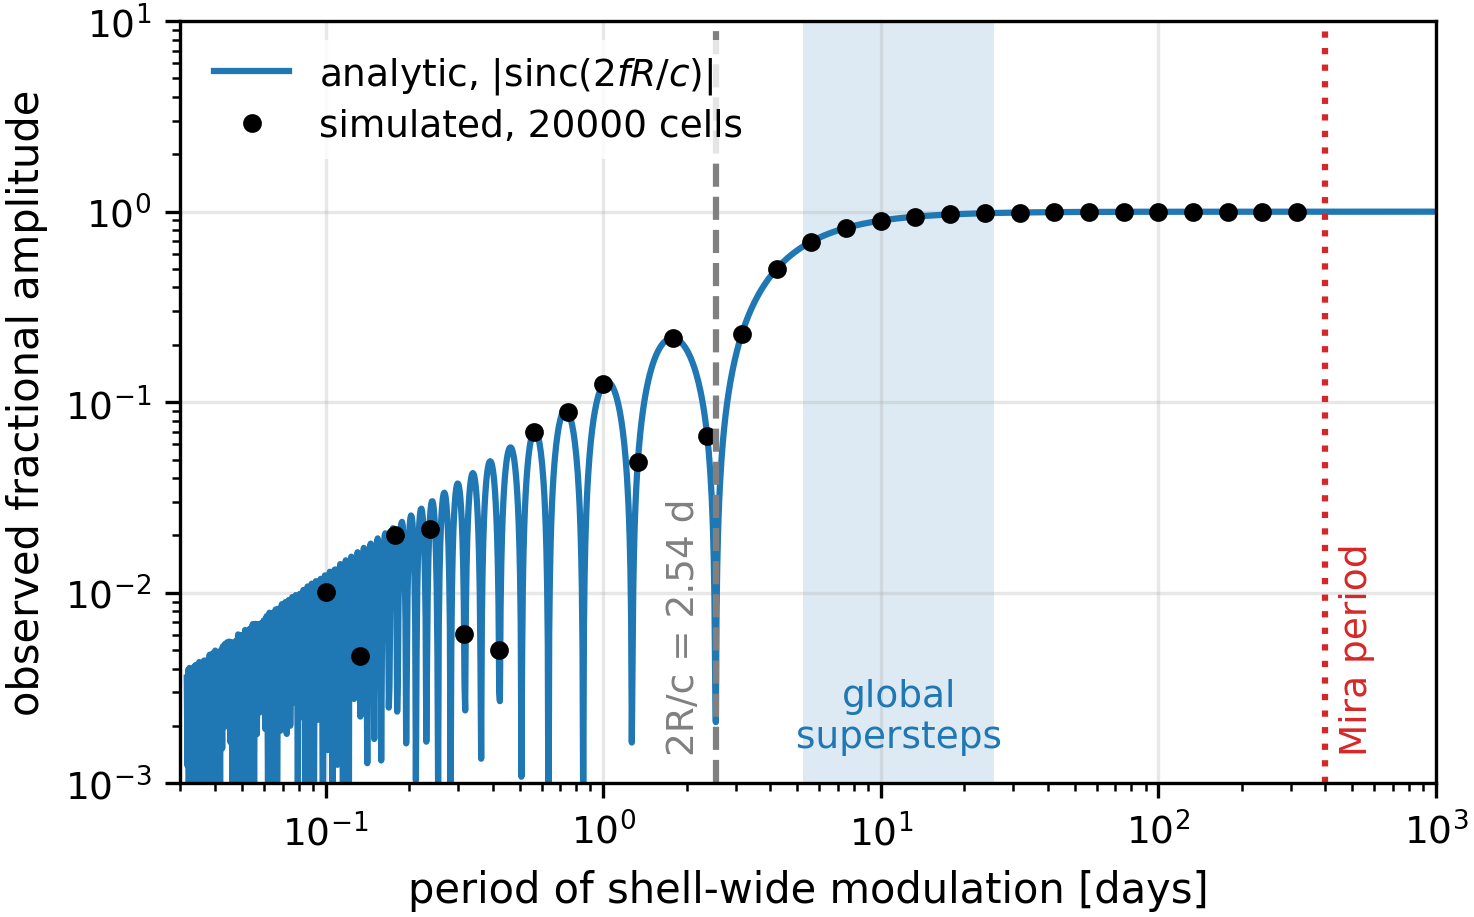
\includegraphics[width=\figwidth]{fig6_light_travel_filter.png}
\caption{Fractional amplitude of a sinusoidal modulation that is simultaneous across the shell, as seen by an unresolved observer. Points: simulated over 20{,}000 cells. Line: Eq.~\eqref{eq:transfer}, the monopole term of Eq.~\eqref{eq:kernel}. The shaded band spans the global superstep cadence, from the 5.3\,d light-crossing bound for a dense hub backbone, through 9.4\,d for 24 hubs, to 26\,d over the mesh (\S\ref{sec:workloads}). Activity that is independent from cell to cell, such as a population of minds, is not filtered but averages away (\S\ref{sec:incoherent}).}
\label{fig:filter}
\end{widefigure}

\begin{widefigure}
\centering
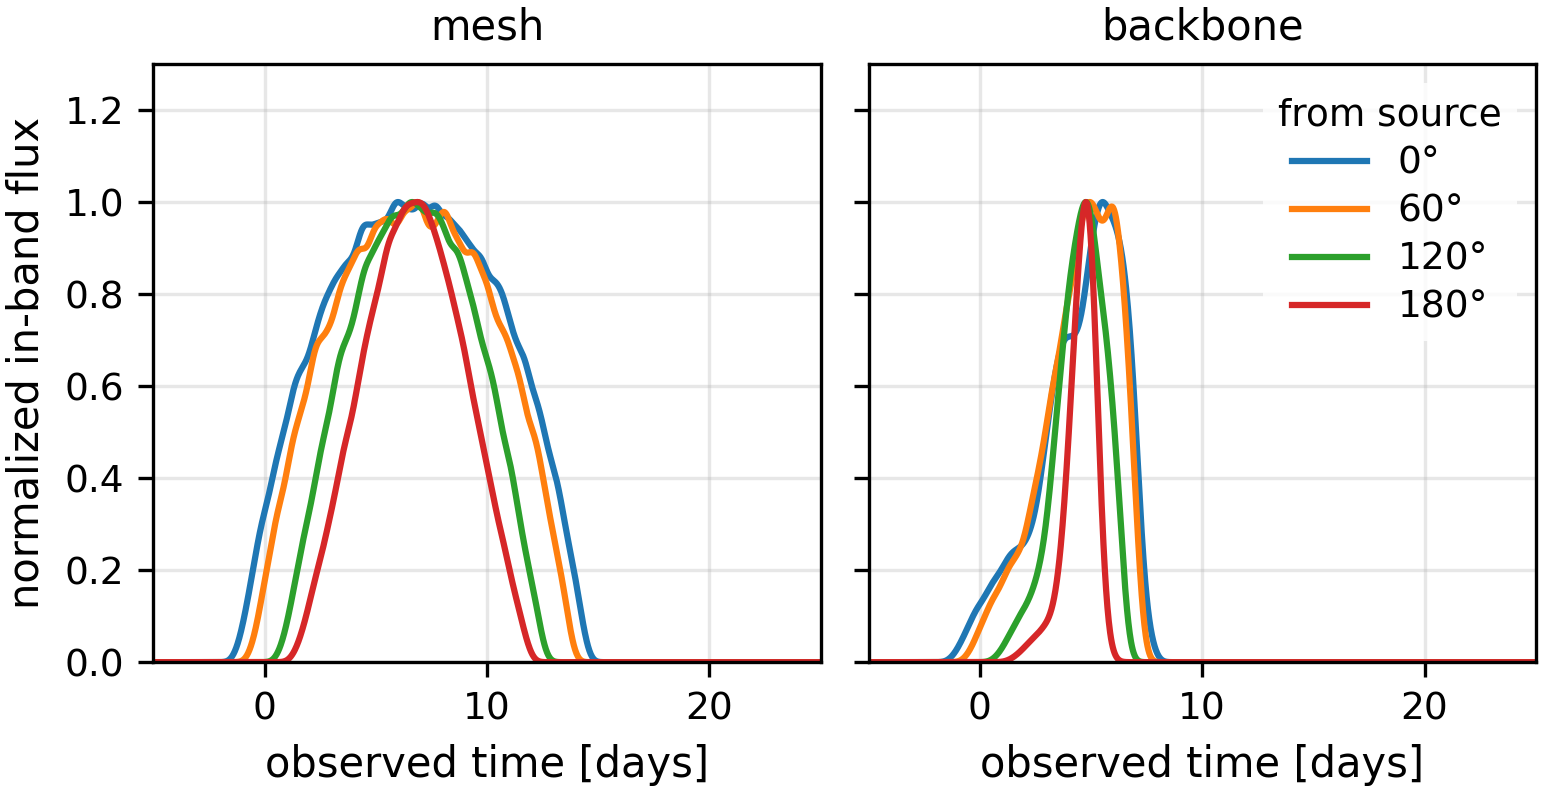
\includegraphics[width=\figwidth]{fig5_broadcast_lightcurves.png}
\caption{Unresolved communication-band light curves of a single broadcast in the millimeter design, for observers at several angles from its source, over a mesh alone (left) and a mesh plus backbone hubs (right).}
\label{fig:lightcurves}
\end{widefigure}

With $2R/c=2.54$\,d, a 1\,d global clock keeps only 12\% of its amplitude, while the 400\,d Mira modulation passes through unattenuated (Fig.~\ref{fig:filter}). A single broadcast produces a communication-band burst with FWHM of 6--12\,d over a millimeter mesh and 1.3--4\,d with a backbone (Fig.~\ref{fig:lightcurves}). Bursts lasting between $2R/c$ and $P_{\rm Mira}$ fall in a time-domain window that natural envelopes have no obvious mechanism to fill coherently.

\subsection{Detectability}

\begin{widetable}
\centering
\caption{Predicted flux densities (Jy) and angular diameters. For reference, WISE reaches 5$\sigma$ point-source sensitivities of 1 and 6\,mJy at 12 and 22\,$\mu$m \citep{Wright2010}, and ALMA's long baselines resolve 0.025$''$ at 0.87\,mm \citep{ALMA2015}.}
\label{tab:det}
\small
\begin{tabular}{lcccccc}
\toprule
$d$ [kpc] & $\theta$ [$''$] & $F_{12\,\mu{\rm m}}$ & $F_{22\,\mu{\rm m}}$ & $F_{850\,\mu{\rm m}}$ & mm comm. & near-IR comm. \\
\midrule
0.5 & 0.88  & 380  & 1370 & 9.2   & 0.78  & 0.034 \\
1.0 & 0.44  & 95   & 342  & 2.3   & 0.19 & 0.0085 \\
3.0 & 0.15  & 10.6 & 38   & 0.26  & 0.022 & 0.0009 \\
8.0 & 0.055 & 1.5  & 5.3  & 0.036 & 0.0030 & 0.00013 \\
\bottomrule
\end{tabular}
\end{widetable}

Black Clouds are bright throughout the Galaxy at mid-infrared, sub-mm and mm wavelengths (Table~\ref{tab:det}). Even at 8\,kpc their 22\,$\mu$m flux exceeds the WISE 5$\sigma$ limit by three orders of magnitude, and their 0.055$''$ diameter spans two beams of ALMA's long baselines, so the shell can be resolved throughout the Galaxy. Detection is not the limiting factor; discrimination is. The WISE prototype of \citet{LaughlinAdams2021}, WISE~J062157.00$-$685659.0 in the Large Magellanic Cloud, illustrates the problem. Its WISE and IRAS colors correspond to blackbodies of 125 to 400\,K, but the authors judge that it is most likely an extremely obscured carbon star.

%======================================================================
\section{Discussion}\label{sec:discussion}
%======================================================================

\subsection{Observing strategy}
\begin{enumerate}
\item \textbf{Select} luminous ($\gtrsim10^3\,\Lsun$), WISE-red sources peaking near 15--20\,$\mu$m, prioritizing AGB and post-AGB hosts.
\item \textbf{Measure the sub-mm spectral index}: $\alpha\approx2$ indicates a gray emitter, $\alpha\approx3$ ordinary dust.
\item \textbf{Search for band-limited excesses.} Use broadband ALMA scans for flat-topped millimeter plateaus with one-sidedly smeared edges and no molecular identification. Use near-infrared spectroscopy (e.g.\ JWST NIRSpec) of the residual stellar light for 10\%-wide, sharp-edged excesses at the 10\% level, the signature of efficient optical-band links.
\item \textbf{Monitor in the time domain}: the candidate bands on day-to-week cadence for bursts with $2R/c\lesssim\Delta t\lesssim P_{\rm Mira}$, and the mid-infrared across a Mira cycle for achromatic variability.
\end{enumerate}
NEOWISE's multi-epoch photometry at 3.4 and 4.6\,$\mu$m \citep{Mainzer2014} lies on the Wien tail of a 177\,K emitter and cannot test the achromaticity criterion. Interferometric positions should precede spectral follow-up, given the background-galaxy confusion that affected Hephaistos \citep{Ren2024,Blain2024,Zackrisson2026}.

\subsection{Time-domain signatures of incoherent cells}\label{sec:incoherent}
The timing search of \citet{Guillochon2026} looked for one coherent clock pushed by discrete kicks. A Black Cloud offers nothing of that kind. Its $\sim10^{28}$ cells leak traffic with independent phases, so the observable is a stochastic excess whose power spectrum has to be compared with the one that the model predicts. Equation~\eqref{eq:transfer} generalizes to arbitrary activity on the shell. If the leak brightness has statistically isotropic angular power $C_\ell(f)$ at temporal frequency $f$, the plane-wave expansion of the light-travel phase gives the spectrum that an unresolved observer receives,
\begin{equation}
S_{\rm obs}(f) = 4\pi R^4\sum_\ell (2\ell+1)\,C_\ell(f)\,j_\ell^2\!\left(\frac{2\pi fR}{c}\right),
\label{eq:kernel}
\end{equation}
where $j_\ell$ is the spherical Bessel function and the monopole term $j_0^2$ recovers Eq.~\eqref{eq:transfer}. We checked the per-mode transfer against direct quadrature and the uncorrelated case against a 20{,}000-cell Monte Carlo. Three properties follow.

First, activity that is uncorrelated from cell to cell is not filtered at all. Since $\sum_\ell(2\ell+1)j_\ell^2(x)=1$ for every $x$, light travel only rearranges incoherent power among multipoles. Incoherent cells are nonetheless invisible, because their summed fluctuation scales as $N^{-1/2}$, about $10^{-14}$ of the leaked power for the optimal design. Only activity correlated over a substantial fraction of the shell can be detected, so a time-domain search measures the low-$\ell$ part of $C_\ell$, not the cells themselves.

Second, temporal frequency maps to angular scale. At frequency $f$ the kernel passes multipoles $\ell\lesssim2\pi fR/c$, which is $\ell\approx8f$ for $f$ in d$^{-1}$ at $R=220$\,AU.

Third, relay causality restricts coordinated power to low frequencies. A correlated pattern on scale $\ell$ cannot be reorganized faster than its relay crossing time, about $\pi R/(\ell v)$, so its power lies at $f\lesssim\ell v/\pi R$, while the kernel requires $f\gtrsim\ell c/2\pi R$. Both conditions can hold only for $v\gtrsim c/2$. The meshes of \S\ref{sec:prop} relay at $0.31c$ to $0.38c$, so their coordinated power at $\ell\ge1$ arrives in the evanescent part of the kernel. What survives is $\ell\lesssim2$ below $v/\pi R$: 0.08 to 0.1\,d$^{-1}$ for a mesh (periods longer than 10 to 13\,d) and about 0.25\,d$^{-1}$ (4\,d) for backbone hubs relaying near $c$. The global supersteps of \S\ref{sec:workloads}, 9.4\,d over the backbone and 26\,d over the mesh (0.11 and 0.04\,d$^{-1}$), fall inside this range. These frequencies lie below the first null of Eq.~\eqref{eq:transfer} at $c/2R=0.39$\,d$^{-1}$, so the comb of nulls is not a usable fingerprint. If the coordinated activity has no schedule, its signature is a low-pass excess whose corner frequency is set by the relay speed and by the radius already fixed from the infrared spectral energy distribution. If it follows the supersteps, the excess concentrates into a quasi-periodic train of broadcast bursts at the superstep cadence. Above about 0.4\,d$^{-1}$ the model predicts nothing beyond the incoherent floor, so fast cadence adds nothing; long, unbroken baselines are what count.

The amplitude of a superstep signal depends on scheduling rather than on the light-travel kernel. At the full bisection rate, global exchange occupies 48\% of the mesh's link capacity along mean great-circle paths, against 20\% for cell-level traffic at $\beta=10^{-6}$. If exchange is confined to a phase of each superstep and idle links fall dark, up to 70\% of the link traffic, and of the leak that follows it, swings once per superstep, so $\epsilon\approx0.5$. If global exchange runs at the bisection rate throughout, as the superstep accounting of \S\ref{sec:workloads} assumes, or idle links carry filler symbols, the leak is steady and $\epsilon\to0$. Because bandwidth is the scarce resource of every design in Table~\ref{tab:optima}, an efficient machine would tend to keep its links saturated, which favors small $\epsilon$. That is an inference about design choices, not a result of the model.

\subsection{Constraints from existing photometry}\label{sec:tess}
The near-infrared communication band of the optimal designs, 0.95--1.05\,$\mu$m, overlaps the red edge of the 600--1000\,nm TESS bandpass \citep{Ricker2015}. With an approximate response curve, the band carries a third of the peak TESS response, and a 2800\,K host puts 21\% of its luminosity into the TESS band. Table~\ref{tab:tess} lists the resulting leak as a fraction of the TESS flux. The observed fluctuation is that fraction multiplied by $\epsilon$, the fractional rms of the cloud-wide coordinated activity, and by the kernel of Eq.~\eqref{eq:kernel}. A fully enclosed host is 5.8\,mag fainter in the optical than its bare star, so the Miras that appear bright to TESS can only be partially covered ($f_{\rm c}\lesssim0.5$), and for them the leak is $6\times10^{-5}$ to $2\times10^{-3}$ of the flux before the factor $\epsilon$ is applied.

\begin{widetable}
\centering
\caption{Communication-band leak as a fraction of the TESS-band flux of a 2800\,K host, for leak fractions of $L_\ast$ from Table~\ref{tab:optima}, as a function of covering fraction. The last row gives the optical dimming of the host by the shell.}
\label{tab:tess}
\small
\begin{tabular}{lccc}
\toprule
 & $f_{\rm c}=0.995$ & $f_{\rm c}=0.5$ & $f_{\rm c}=0.1$ \\
\midrule
$\beta=10^{-6}$ & $1.3\times10^{-2}$ & $6.4\times10^{-5}$ & $7.1\times10^{-6}$ \\
$\beta=10^{-4}$ & 0.39 & $1.9\times10^{-3}$ & $2.2\times10^{-4}$ \\
host dimming (mag) & 5.8 & 0.8 & 0.1 \\
\bottomrule
\end{tabular}
\end{widetable}

To see what current data allow, we cross-matched the 3435 Miras in the International Variable Star Index \citep{Watson2006} that are brighter than $V=11$ at maximum with the TESS Input Catalog. Of the 3403 matches, 122 have targeted two-minute light curves and 36 lie in the continuous viewing zones near the ecliptic poles, where TESS returns every year. In R~Ret, the most observed (31 sectors), the simple-aperture photometry of 12 contiguous sectors reaches 4--5\,ppm per frequency bin above 10\,d$^{-1}$ after the pulsation is removed, but 120\,ppm at 0.1--0.4\,d$^{-1}$, where Mira-cycle residuals and spacecraft systematics dominate. That is the window in which coordinated activity would appear, and a single-band spectrum cannot separate a 10--100\,ppm low-pass excess from the star's own red noise.

A second band removes that degeneracy. Stellar variability appears in TESS and in a simultaneous bluer band with a fixed transfer ratio, whereas the leak adds power only to the band containing 1\,$\mu$m. A deficit of cross-band coherence below the corner frequency would therefore reveal the leak without a model of the stellar noise. We tested this on X~Dra, a Mira in the continuous viewing zone with eight contiguous sectors of 200\,s full-frame photometry \citep{Caldwell2020} and simultaneous ZTF $g$ and $r$ epochs \citep{Bellm2019}. After a joint fit of the Mira cycle, the TESS residual is 3\,mmag, but the ZTF residuals are 14--19\,mmag, close to their photometric errors. No significant coherence is found between the bands (permutation $p=0.09$--$0.74$), so the second band cannot be used to remove the stellar noise. Injections of the model excess (Eq.~\eqref{eq:kernel} with $v=0.38c$) show that the cycle fit absorbs 57\% of the injected variance, because the corner frequency falls near the 13.7\,d TESS orbit, and that an excess becomes detectable at about 4000\,ppm rms. Trains of bursts at the superstep cadence fare differently for the backbone and the mesh. A search of the periodogram for a line recovers half of the 9.4\,d backbone trains at about 1000\,ppm rms. The cycle fit leaves 83\% of their variance, because 0.11\,d$^{-1}$ falls between the first two harmonics of the TESS orbit. The 26\,d mesh cadence coincides with a TESS sector and two orbits, so the fit removes 80\% of the signal and detection needs about 8000\,ppm. The deepest of these bounds limits $\epsilon$ times the leak fraction to below about $10^{-3}$, and it reaches only the fully enclosed rows of Table~\ref{tab:tess}. A host with $f_{\rm c}=0.995$, $\beta=10^{-6}$ and phased exchange would sit near 6000\,ppm, but it would be 5.8\,mag fainter than the bright Miras that TESS monitors. A detection in a single bright Mira is therefore not expected, because the hosts that TESS sees well cannot be enclosed.

We then searched the whole TESS Mira population for the superstep burst train. Of the 81,453 Miras in the International Variable Star Index, 48,550 match a TESS Input Catalog star brighter than $T=14$, which includes the optically faint, red Miras left out above. Of these, 6148 have a two-minute or 200\,s full-frame light curve, giving 7885 segments of at least 20\,d from 6108 stars. In each segment we removed the Mira cycle as for X~Dra and searched the residual periodogram for a line at 3--30\,d. The fundamental carries 87\% of a burst train's detectable power. The spacecraft also leaves lines of its own at harmonics of the 13.7\,d orbit and at the momentum-dump cadence. We therefore calibrated the significance empirically, frequency by frequency, against every Mira observed on the same camera in the same sector. With this null the bulk of the sample matches the expected false-alarm counts: 910 segments lie below a false-alarm probability of 0.1, against 789 expected.

Forty segments from 38 stars carry a line that is significant across the whole population, and none of them points to a cloud. Ten have a cataloged periodic neighbor at the line's period or a harmonic, found in VSX or Gaia DR3 \citep{Vallenari2023}. Most of the rest are shared with other stars in the same sector, fit dips better than bursts, or fail to recur in the star's other sectors. Of the four stars that pass every time-domain test, one (NSVS~J2213225+733019) is a Mira-cycle residual in a segment where the star moved by 2.1\,mag. In the full-frame pixels, the line of NGCA-V6 coincides with a $G=15.5$ neighbor $53''$ away, that of V0621~Herculis is the dipole of a moving image rather than a change in brightness, and that of CGCS~6098 is not reproduced by independent photometry.

Injections of burst trains into 800 random segments set the depth of the search. For superstep periods of 3--6\,d, half of the trains are recovered at a median of 1700\,ppm rms, and at 550\,ppm in the quietest quarter of segments. The population search therefore excludes $\epsilon$ times the leak fraction above about $2\times10^{-3}$, or $6\times10^{-4}$ for the quietest quarter. That reaches the fully enclosed host with phased exchange in Table~\ref{tab:tess} in about 6000 Miras, if its superstep falls in that range. At longer periods the per-orbit systematics absorb the signal. At the 9.4\,d backbone superstep of the fiducial 220\,AU host, only about 30\% of 3000\,ppm trains are recovered. Since a superstep scales as $R/c\propto L_\ast^{1/2}$, only hosts fainter than about $800\,\Lsun$ place it in the well-covered band. The partially covered hosts that dominate the sample remain below this limit, since their leak is at most $2\times10^{-3}$ of the flux before the factor $\epsilon$. The data products and scripts are in \texttt{research/tess-spectral-search.md} and \texttt{util/tess/}.

\subsection{Survey requirements}\label{sec:surveys}
The analysis above sets three requirements on a survey that could detect the time-domain leakage, or rule it out.
\begin{enumerate}
\item \textbf{Optically faint, infrared-bright hosts.} Enclosed hosts carry the largest leak fraction, 12\% of the escaping starlight within the band (\S\ref{sec:leak}) and 1.3\% across the TESS bandpass at $\beta=10^{-6}$, but are much fainter than the bright samples monitored today. The Vera C. Rubin Observatory's LSST is well matched to such sources: its $ugrizy$ filters reach 1050\,nm and saturate near $r\sim16$ \citep{Ivezic2019}. Its $y$ band contains the communication band and its $z$ band does not, so a time series of the $z-y$ color of WISE-red, optically faint AGB candidates compares in-band with out-of-band flux at the multi-day cadence that the corner frequencies of \S\ref{sec:incoherent} require.
\item \textbf{Spectral resolution across the band edge.} SPHEREx observes 0.75--5\,$\mu$m, at a resolving power of about 40 below 3.8\,$\mu$m \citep{Dore2014, Crill2020}, or 25\,nm at 1\,$\mu$m, which resolves a 10\%-wide band with sharp edges. Its deep fields, about 100\,deg$^2$ near each ecliptic pole and revisited on every orbit \citep{Crill2020}, overlap the TESS continuous viewing zones. Repeated spectra there can track the ratio of in-band to out-of-band flux directly, and simultaneous TESS light curves add the fine time sampling.
\item \textbf{A millimagnitude reference band and shared systematics models.} The cross-band coherence test works only when the reference band's noise lies below the stellar fluctuation it shares with TESS. That requires nightly photometry of the Miras in the continuous viewing zones, in a band bluer than 0.9\,$\mu$m and at about 1\,mmag, roughly five times better than ZTF achieves on X~Dra. ATLAS \citep{Tonry2018}, ASAS-SN \citep{Shappee2014,Hart2023} or a dedicated small telescope could provide it. The TESS orbit and its scattered-light ramps fall inside the predicted window, so systematics should be fit jointly for all Miras on a camera rather than absorbed star by star.
\end{enumerate}
None of these surveys is needed to find a Black Cloud candidate in the first place; the static tests of the observing strategy above do that. They are what would turn a candidate into a test of whether its communication band carries computational state.

\subsection{Minds as a workload}\label{sec:minds}
Section~\ref{sec:workloads} describes the kinds of computation that fit a Black Cloud, not what a civilization would want from one. One answer that fits the hierarchy unusually well is the emulation of minds. If minds are computational processes, as the literature on whole-brain emulation assumes \citep{Eth2013,Hanson2016}, a Black Cloud is less a calculating engine than a place for minds to live. The numbers below assume emulation at the level of individual synapses. Other levels of biological detail would move them by orders of magnitude.

\emph{Cost of one mind.} The adult human brain has $8.6\times10^{10}$ neurons \citep{Azevedo2009}, and its neocortex alone has $1.6\times10^{14}$ synapses \citep{Tang2001}. The brain's energy budget allows fewer than 1\% of cortical neurons to be strongly active at once \citep{Lennie2003}. If an active neuron fires at up to 50\,Hz (an assumption), the mean rate is at most 0.5\,Hz and the neocortex handles at most $8\times10^{13}$ synaptic events per second. Charging one multiply--add, $3\times10^4$ bit operations (\S\ref{sec:beta}), per event gives $2.5\times10^{18}$ bit operations per second for real-time emulation. Mean rates down to 0.1\,Hz and $10^4$--$10^5$ bit operations per event widen this to $1.6\times10^{17}$--$8\times10^{18}$. At the Landauer limit and 177\,K the emulation dissipates 4\,mW, about 5000 times less than the 20\,W the brain draws \citep{Levy2020}. An energy audit of the brain points the same way: its neurons operate about $10^8$ times above the best possible bits per joule \citep{Levy2021}.

\emph{Communication.} A mind is a natural cell-level workload. Shipping every spike as an address of $\log_2(8.6\times10^{10})\approx36$ bits takes $1.6\times10^{12}$\,bit\,s$^{-1}$, or $6\times10^{-7}$ bits per bit operation of the emulation. That is essentially the fiducial $\beta=10^{-6}$ that we inferred independently from terrestrial supercomputers in \S\ref{sec:beta}, and in the cortex itself communication already costs 35 times as much energy as computation \citep{Levy2021}. A brain, a supercomputer and an optimally built Black Cloud thus share one communication budget. A fiducial node can run about seven minds in real time (2 to 110 over the range above), and their spike traffic would use 3\% of its link capacity. The rest, about $5\times10^{13}$\,bit\,s$^{-1}$ per mind, is available for exchange between minds, $10^{12}$ times the 39\,bit\,s$^{-1}$ that human speech carries \citep{Coupe2019}.

\emph{Population.} At real-time speed a cell hosts about $10^4$ minds and the whole cloud about $2\times10^{32}$ ($5\times10^{31}$ to $3\times10^{33}$). Its $1.4\times10^{62}$ lifetime bit operations provide $2\times10^{36}$ mind-years of subjective experience, however they are divided between more minds and faster ones.

\emph{Subjective time and the shape of society.} A mind alone on a node runs about seven times faster than biology. Spreading it across nodes makes it faster, until each relay hop (1.6\,$\mu$s) becomes comparable to the shortest timescale that the emulation must resolve. Taking that to be 1\,ms gives a ceiling of about 600 times real time, reached on about 85 nodes, well inside one cell. At that speed a global superstep of 9.4\,d lasts 16 subjective years, and a message to the far side of the shell takes eight. \citet{Hanson2016} argued that latency would pull fast emulations into dense cities. In a Black Cloud the same pressure is built into the geometry: a cell is a town of $10^4$ minds that share a $20\,\mu$s neighborhood, while the shell as a whole is a federation of $10^{28}$ such towns whose collective decisions take subjective years. A civilization of minds is therefore the same archipelago as the computer it runs on.

\emph{Detectability.} A society of minds is close to the quietest workload a Black Cloud could run. Each mind's traffic stays within a node or a cell, and $10^{28}$ independent cells leak power whose fluctuations average down as $N^{-1/2}$ (\S\ref{sec:incoherent}). Only activity coordinated across the whole shell, such as synchronized exchange in global supersteps, would modulate the communication band at the days-to-weeks periods of \S\ref{sec:workloads}. A civilization of minds absorbed in its own affairs would show its waste heat and its static communication band, but no time-domain signature of what it is thinking. This is the waste-heat analog of the conclusion of \citet{Guillochon2026}, that efficient communication is indistinguishable from noise.

\emph{Adaptation to the Mira cycle.} The stellar pulsation is the one rhythm that the whole cloud shares without communicating, and no store can absorb its $\pm40\%$ swing (\S\ref{sec:thermal}). At 850\,$\mu$m a passive shell varies by $\pm11\%$, close to the $\pm9\%$ of our toy dust envelope, but a thermostatted shell varies by $\pm40\%$. How the millimeter plateau of the communication band varies relative to the adjacent continuum depends on how the civilization shares the fluctuating budget (Fig.~\ref{fig:minds-mira}). If a passive shell lets traffic follow the available power, the plateau-to-continuum ratio swings by $\pm31\%$ in phase with the star. If a thermostatted shell holds its minds' traffic steady, the ratio swings by $\pm40\%$ in anti-phase. The other two combinations leave the ratio nearly constant. The phase of the sub-mm continuum itself is not a safe discriminant, since the 850\,$\mu$m peak of IRC+10216 trails its optical peak by about 540\,d for reasons only partly understood \citep{Dharmawardena2019}. The plateau-to-continuum ratio is better, since natural molecular lines need not follow the star: the $^{12}$CO(3--2) line of IRC+10216 shows no periodic variation even at the 10\% level \citep{Dharmawardena2019}.

\begin{widefigure}
\centering
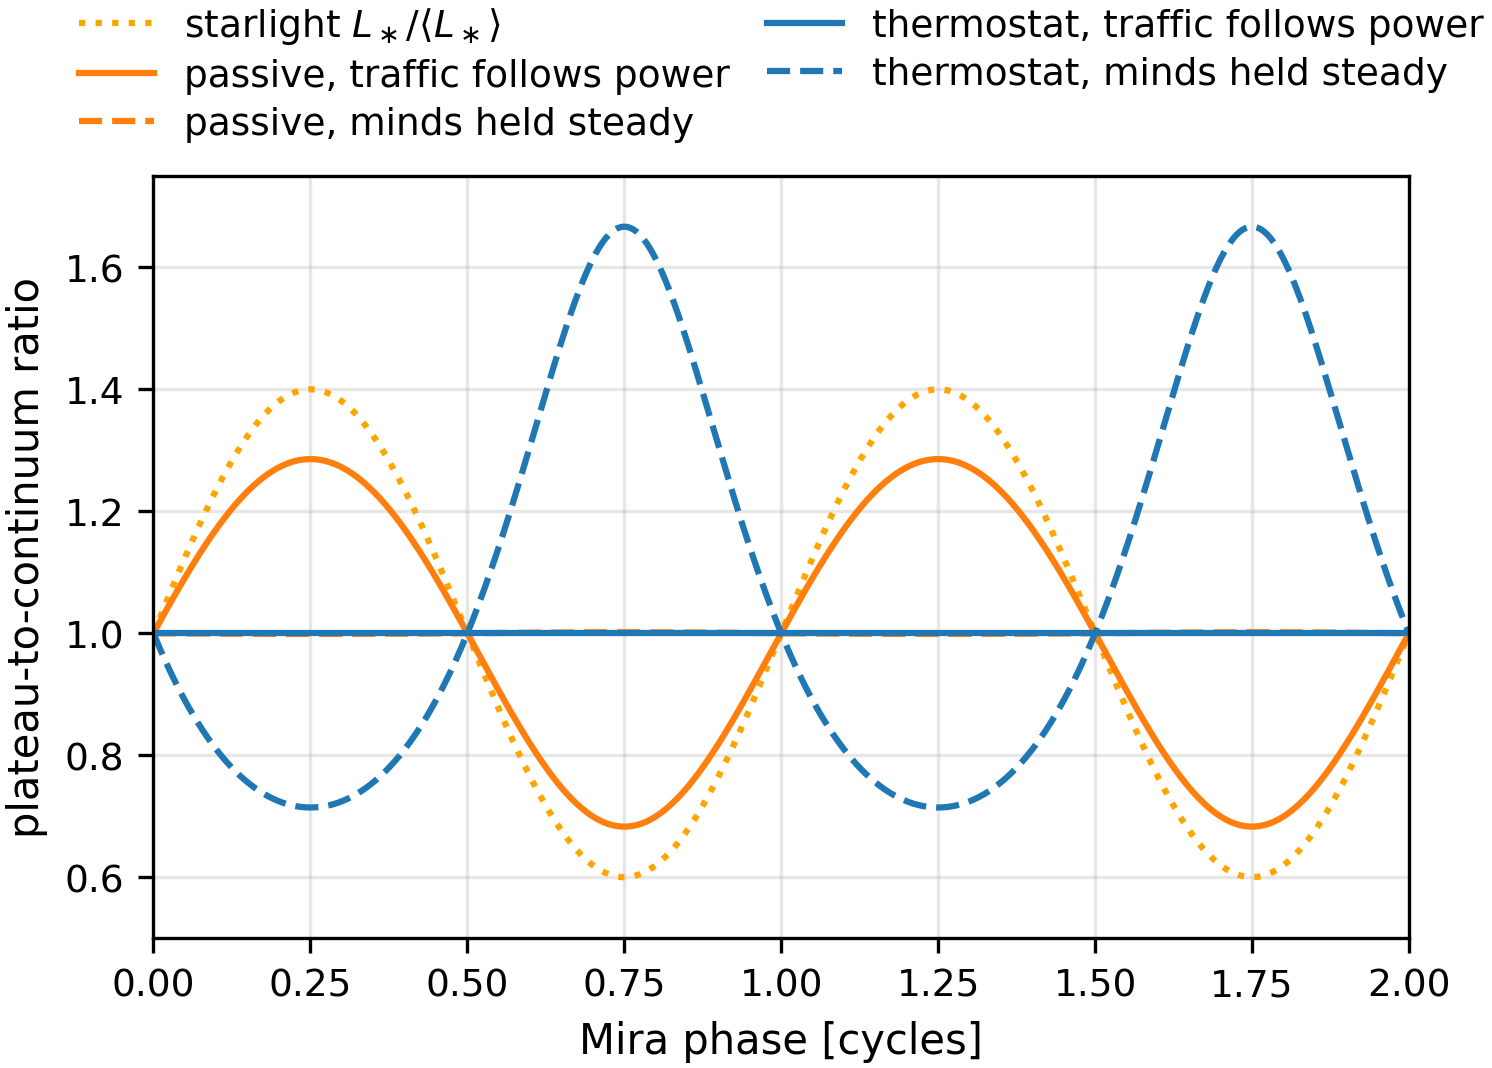
\includegraphics[width=\figwidth]{fig12_mind_scheduling.png}
\caption{Ratio of the millimeter communication plateau to the adjacent continuum over two Mira cycles, normalized at mean luminosity, for a passive (orange) or thermostatted (blue) shell whose traffic either follows the available power (solid) or is held steady for its minds (dashed). Dotted: the stellar luminosity. Light travel delays plateau and continuum equally and drops out of the ratio. Two cases leave the ratio within 1\% of constant and overlap at unity.}
\label{fig:minds-mira}
\end{widefigure}

\subsection{Limitations}
The model is intentionally minimal. The shell is spherically symmetric and uniformly filled, with no clumping or Matryoshka layering. Its outflow dynamics are ignored, although homologous expansion stretches tangential links and so offers a physical reason for periodic rebuilding. The natural envelopes are optically thin with a single emissivity index, without solid-state features. Links are idealized Fresnel-matched apertures with the noise floor of coherent detection. \citet{LaughlinAdams2021} rejected carriers shorter than about 1\,mm because the dust grains absorb them. Our near-infrared designs assume that the grains between nodes have been built into the structure, so that the only opacity is the covering $\tau$ of the nodes themselves. Photon-counting receivers could carry several bits per photon in the quantum regime, and multimode near-field links ($d<A/\lambda$) raise $\sigma_b$ as the square root of the mode number, at the cost of the short hops and fault tolerance of a mesh. The bits-per-operation ratio $\beta$ is inferred from terrestrial machines. The mind-hosting estimates of \S\ref{sec:minds} assume that minds are computational and can be emulated at the level of synapses; both assumptions are open questions. Most importantly, the design choices (carrier, $\beta$, thermostatting, backbone) dominate the uncertainty. The model maps each choice to its observable consequences rather than predicting what an engineer would choose.

%======================================================================
\section{Conclusions}
%======================================================================
\begin{enumerate}
\item A Black Cloud has a natural computing cell,
\[
\lcell=\frac{2\tau f_B c\,\kTl}{\beta F\lambda^2}.
\]
Its size is set by the carrier wavelength, independent of lattice and shell thickness, and it carries a characteristic time, frequency and energy.
\item Millimeter links give the structure about $10^{9}$ times less bandwidth per operation than a supercomputer. An efficient design uses near-infrared links between centimeter-scale nodes on a high-radix (FCC) lattice, forming kilometer-scale cells that tick at about 50\,kHz. Each 0.34\,g, 43\,W cell has roughly half the throughput of El Capitan, the second-fastest terrestrial supercomputer, assuming Landauer-limited operation.
\item Infrared waste heat traces the star, not the computation. Sub-mm spectral slope and, for thermostatted designs, achromatic variability are the useful thermal discriminants.
\item Internal communication is the only leakage channel that carries computational state. It appears as a 3\,mm plateau of about 0.2\,Jy at 1\,kpc for the original design, or a 10\%-level, sharp-edged band on the escaping starlight for an optimized one.
\item Light-travel smoothing over $2R/c$ defines a time-domain window for coherent computational activity, complementary to the timing searches of pulsating stars.
\end{enumerate}

\section*{Data availability}
The model (\texttt{blackcloud/}) and the scripts that regenerate every figure and number in this paper (\texttt{run\_model.py}, \texttt{run\_cells.py}) are available at \url{https://github.com/guillochon/blackcloud}.

\section*{Declaration of generative AI and AI-assisted technologies in the manuscript preparation process}
During the preparation of this work the author used Claude (Anthropic) to draft and edit text, derive and check analytic results, and write the modeling and figure-generation code. The figures are produced by that code; no generative model created or altered plotted data. After using this tool, the author reviewed and edited the content as needed and takes full responsibility for the content of the published article.

\section*{Declaration of competing interest}
The author declares no competing financial interests or personal relationships that could have appeared to influence the work reported in this paper.

\section*{CRediT authorship contribution statement}
\textbf{James Guillochon:} Conceptualization, Methodology, Software, Writing -- original draft, Writing -- review \& editing.

\bibliographystyle{elsarticle-num-names}
\bibliography{refs}

\end{document}
